\subsection{利用三角形式进行复数的乘方运算}

现在我们研究$n$个复数相乘的问题。

设$z_k=r_k(\cos\theta_k+i\sin\theta_k),\quad k=1,2,3,\ldots,n$。利用数学归纳法容易证明
\[z_1\cdot z_2\cdots z_n=r_1\cdot r_2\cdots r_n\left[\pcx{\theta_1+\theta_2+\cdots+\theta_n}\right]\]

特别是当$z_1= z_2=\cdots= z_n$时,即
\[r_1=r2=\cdots=r_n=r,\qquad \theta_1=\theta_2=\cdots=\theta_n=\theta\]
代入上式就有
\[[r(\pc{\theta})]^n=r^n(\pc{n\theta})\quad (n\in\N)\]
这就是说,
\textbf{复数$z$的$n\; (n\in\N)$次幂,其模等于$z$的模的$n$次幂,其辐角等于$z$的辐角的$n$倍}。
这就是著名的\textbf{棣莫佛\footnote{棣莫佛(Abraham de Moivre)1667--1754年,法国数学家.}定理}。

\begin{example}
计算$\left(\sqrt{3}-i\right)^6$
\end{example}

\begin{solution}
先把$\sqrt{3}-i$化为三角形式,再利用棣莫佛定理
\[\begin{split}
\left(\sqrt{3}-i\right)^6=\left[2\left(\pc{\frac{11\pi}{6}}\right)\right]&=2^6(\pc{11\pi})\\
&=64(\pc{\pi})=64(-1)=-64
\end{split}\]
\end{solution}


\begin{example}
    计算
\begin{multicols}{2}
\begin{enumerate}[(1)]
    \item $\left(-\frac{1}{2}+\frac{\sqrt{3}}{2}i\right)^3$
    \item $\left(-\frac{1}{2}-\frac{\sqrt{3}}{2}i\right)^3$
\end{enumerate}
\end{multicols}
\end{example}

\begin{solution}
\begin{enumerate}[(1)]
    \item $\left(-\frac{1}{2}+\frac{\sqrt{3}}{2}i\right)^3=\left(\pc{\frac{2\pi}{3}}\right)^3=\pc{2\pi}=1$
    \item $\left(-\frac{1}{2}-\frac{\sqrt{3}}{2}i\right)^3=\left(\pc{\frac{4\pi}{3}}\right)^3=\pc{4\pi}=1$
\end{enumerate}
\end{solution}

\begin{example}
下列哪种算法是正确的:

算法1:\[\begin{split}
    \left(\frac{-1+\sqrt{3}i}{2}\right)^{10}&=\left[\left(\frac{-1+\sqrt{3}i}{2}\right)^3\right]^3\left(\frac{-1+\sqrt{3}i}{2}\right)\\
    &=1^3 \cdot \left(\frac{-1+\sqrt{3}i}{2}\right)=\frac{-1+\sqrt{3}i}{2}
\end{split}\]
算法2:
\[\left(\frac{-1+\sqrt{3}i}{2}\right)^{10}=\left[\left(\frac{-1+\sqrt{3}i}{2}\right)^8\right]^{\tfrac{10}{8}}=1^{\tfrac{10}{8}}=1\]
\end{example}

\begin{solution}
算法1是正确的。这说明在复数集中$(z^n)^m=2^{mn},\quad m,n\in\Z$,而$m$,$n$不能为分数。
\end{solution}


\begin{example}
    若$z=\left(1+\sqrt{3}i\right)^n$,当$n$为哪些正整数时$z\in\R$.
\end{example}

\begin{solution}
$    z=\left(1+\sqrt{3}i\right)^n=\left[2\left(\pc{\frac{\pi}{3}}\right)\right]^n=2^n\left(\pc{\frac{n\pi}{3}}\right)$
\[z\in\R\Leftrightarrow \sin \frac{n\pi}{3}=0 \Leftrightarrow \frac{n\pi}{3}=k\pi\; (k\in\Z)\]

$\therefore\quad n=3k\; (k\in\Z,\; n\in\N)$

$\therefore\quad $当$n$为$3k\; (k\in\N)$时,$z\in\R$.
\end{solution}
    
\begin{example}
计算$(1+i\tan\theta)^n$,其中$\frac{\pi}{2}<\theta<\pi$
\end{example}

\begin{solution}
记$z=1+i\tan\theta=\frac{1}{\cos\theta}(\cos\theta+i\sin\theta)=\frac{-1}{\cos\theta}\left[\pcx{\theta+\pi}\right]$

\[\begin{split}
    \therefore\quad z^n&=\frac{(-1)^n}{\cos^n\theta}\left[\pcx{n\pi+n\theta}\right]\\
    &=\begin{cases}
        \frac{1}{\cos^n \theta}(\pc{n\theta}), & n\text{为偶数}\\[1.5ex]
        \frac{-1}{\cos^n \theta}\left[\pcx{\pi+n\theta}\right], & n\text{为奇数}\\
    \end{cases}
\end{split}\]
\end{solution}

\begin{example}
    求证:两个互为共轭的复数,其$n$次幂仍为共轭复数($n\in\N$)
\end{example}

\begin{proof}
设$z=r(\pc{\theta}),\quad \bar z=r\left[\pcx{-\theta}\right]$
\[\begin{split}
    z^n&=r^n(\pc{n\theta})\\
\bar z^n&=r^n\left[\pcx{-n\theta}\right]=r^n\left(\cos n\theta-i\sin n\theta\right)
\end{split}\]
$\therefore\quad z^n$与$\bar z^{n}$仍为共轭复数.
\end{proof}

\begin{example}
利用复数证明:
\[\sin2\theta=2\sin\theta\cos\theta,\qquad \cos2\theta=\cos^2\theta-\sin^2\theta\]
\end{example}

\begin{proof}
设$z=\pc{\theta}$,一方面,由棣莫佛定理得
\[z^2=(\pc{\theta})^2=\cos2\theta+i\sin2\theta\]
另一方面,由乘法公式得
    \[z^2=(\pc{\theta})^2=\cos^2\theta-\sin^2\theta+2i\cos\theta\sin\theta\]
    比较以上两式,得
    \[\cos2\theta=\cos^2\theta-\sin^2\theta,\qquad \sin2\theta=2\sin\theta\cos\theta\]
\end{proof}

\section*{习题八}
\begin{center}
    \bfseries A
\end{center}

\begin{enumerate}
    \item 计算:
\begin{multicols}{2}
\begin{enumerate}[(1)]
    \item $\left[3\left(\pc{18^{\circ}}\right)\right]^5$
    \item $\left[\sqrt{2}\left(\pc{\frac{\pi}{4}}\right)\right]^6$
    \item $\left[3(\pc{10^{\circ}})\right]^6$
    \item $\left[2(\pc{15^{\circ}})\right]^6$
    \item $(1-i)\left(-\frac{1}{2}+\frac{\sqrt{3}}{2}i\right)^7$
    \item $(1-i)^{10}$
    \item $\left(1+\sqrt{3}i\right)^4$
    \item $\left(2-2\sqrt{3}i\right)^4$
\end{enumerate}
\end{multicols}
    \item 计算:
\begin{multicols}{2}
\begin{enumerate}[(1)]
    \item $\left(-\frac{1}{2}+\frac{\sqrt{3}}{2}i\right)^{101}$
    \item $\left(-\frac{1}{2}-\frac{\sqrt{3}}{2}i\right)^{101}$
\end{enumerate}
\end{multicols}
\end{enumerate}

\begin{center}
    \bfseries B
\end{center}
\begin{enumerate}\setcounter{enumi}{2}
    \item 设$z=\left(-3\sqrt{2}+3\sqrt{2}\right)^n$,当$n$为哪些正整数时,$z\in\R$.
    \item 求证:$\left(\frac{1+i}{\sqrt{2}}\right)^n\left(\frac{1-i}{\sqrt{2}}\right)^n$,当$n$为正偶数时,值为$\pm 2$或0;当$n$为正奇数时,值为$\pm\sqrt{2}$.
    \item 用复数证明三倍角公式:
\[\sin3\alpha=3\sin\alpha-4\sin^3\alpha,\qquad \cos3\alpha=4\cos^3\alpha-3\cos\alpha\]
\item 计算 
\begin{enumerate}[(1)]
    \item 若$2\pi<\theta<3\pi$,计算$(1+\pc{\theta})^n$
    \item $(\tan\theta+i)^5$
\end{enumerate}
\end{enumerate}

\subsection{利用三角形式进行复数的除法运算}
设$z_1=r_1(\pc{\theta_1})$,
$z_2=r_2(\pc{\theta_2})$,$z_2\ne 0$. 
根据6.3节复数除法的定义,有
\[\begin{split}
    z_1\div z_2=\frac{z_1}{z_2}&=\frac{r_1(\pc{\theta_1})}{r_2(\pc{\theta_2})}\\
    &=\frac{r_1}{r_2}\cdot \frac{(\pc{\theta_1})(\cos\theta_2-i\sin\theta_2)}{\cos^2\theta_2+\sin^2\theta_2}\\
    &=\frac{r_1}{r_2}(\pc{\theta_1})\left[\pcx{-\theta_2}\right]\\
    &=\frac{r_1}{r_2}\left[\pcx{\theta_1-\theta_2}\right]
\end{split}\]
即
\[\frac{r_1(\pc{\theta_1})}{r_2(\pc{\theta_2})}=\frac{r_1}{r_2}\left[\pcx{\theta_1-\theta_2}\right]\]
这就是说,\textbf{两个复数相除,商的模等于被除数与除数模的商,商的
辐角等于被除数与除数辐角的差。}

\begin{example}
计算: $4\left(\pc{\frac{4\pi}{3}}\right)\div 2\left(\pc{\frac{5\pi}{6}}\right)$
\end{example}

\begin{solution}
\[\begin{split}
    \text{原式}=\frac{4\left(\pc{\frac{4\pi}{3}}\right)}{2\left(\pc{\frac{5\pi}{6}}\right)}&=2\left[\pcx{\frac{4\pi}{3}-\frac{5\pi}{6}}\right]\\
&=2\left(\pc{\frac{\pi}{2}}\right)=2(0+i)=2i
\end{split}\]
\end{solution}

\begin{example}
计算:$\frac{(\sin\theta-i\cos\theta)^2\cdot (-\cos\theta+i\sin\theta)^3}{(\cos\theta-i\sin\theta)^4}$
\end{example}

\begin{analyze}
须先化成三角形式再乘、除. 原式为:
\[\begin{split}
&\quad \frac{\left[\pcx{\frac{3\pi}{2}+\theta}\right]^2\cdot \left[\pcx{\pi-\theta}\right]^3}{\left[\pcx{-\theta}\right]^4}
\\
&=\frac{\left[\pcx{3\pi+2\theta}\right]\left[\pcx{3\pi-3\theta}\right]}{\pcx{-4\theta}}\\
&=\frac{\pcx{6\pi-\theta}}{\pcx{-4\theta}}\\
&=\pcx{6\pi+3\theta}=\pc{3\theta}
\end{split}\]    
\end{analyze}


\begin{example}
设$z_1=6\left(\pc{\frac{\pi}{3}}\right)$,
$z_2=2\left(\pc{\frac{\pi}{4}}\right)$,试用几何作图的方法,用起点在原点的向量表示$z=z_1\div z_2$
\end{example}

\noindent
\begin{minipage}{.55\textwidth}
\begin{solution}
先作出表示$z_1,z_2$的向量$\vv{OZ_1}$,$\vv{OZ_2}$(图6.25),然后把$\vv{OZ_1}$顺时针旋转$\frac{\pi}{4}$,再把它的模缩为原来的$\frac{1}{2}$,所得向量$\vv{OZ}$表示$z_1\div z_2$. 这就是\textbf{复数除法的几何意义}。这里应特别注意:
\[\text{商的模}=\frac{r_1}{r_2}=\frac{|z_1|}{|z_2|}\]
(这提供了求两复数模的比的有效方法)
\[\text{商的辐角}=\theta_1-\theta_2\]
(这提供了求向量$\vv{OZ_1}$与$\vv{OZ_2}$夹角的方法)
\end{solution}    
\end{minipage}\hfill
\begin{minipage}{.4\textwidth}
\centering
\begin{tikzpicture}[>=stealth, scale=.7]
\draw[->](-1,0)--(5,0)node[below]{$x$};
\draw[->](0,-1)--(0,6)node[left]{$y$};
\node[below left]{$O$};
\draw[very thick, ->](0,0)--(60:6)node[above]{$z_1$};
\draw[very thick, ->](0,0)--(45:2)node[above]{$z_2$};
\draw[very thick, ->](0,0)--(15:3)node[right]{$z$};
\draw[->](3.5,0) arc (0:60:3.5);
\draw[->](2.15,0) arc (0:15:2.15);
\draw[->](60:2.5) arc (60:15:2.5);
\draw[->](1,0) arc (0:45:1);
\node at (30:4){$\tfrac{\pi}{3}$};
\node at (15/2:2.5){$\tfrac{\pi}{12}$};
\node at (45/2:1.25){$\tfrac{\pi}{4}$};
\node at (75/2:2.75){$-\tfrac{\pi}{4}$};


\end{tikzpicture}
\captionof{figure}{}
\end{minipage}

\begin{example}
    已知:$z=\frac{(3-4i)^2\cdot (\sqrt{3}+i)^4}{(1+i)^6}$,求$|z|$.
\end{example}

\begin{analyze}
若将$z$算出,再求$|z|$显然很繁。可直接根据$\left|\frac{z_1}{z_2}\right|=\frac{|z_1|}{|z_2|}$, $|z_1\cdot z_2|=|z_1|\cdot |z_2|$,$|z^n|=|z|^n$去做.    
\end{analyze}

\begin{solution}
$|z|=\left|\frac{(3-4i)^2\cdot (\sqrt{3}+i)^4}{(1+i)^6}\right|=\frac{|3-4i|^2\cdot \left|\sqrt{3}+i\right|^4}{|1+i|^6}=\frac{5^2\cdot 2^4}{\left(\sqrt{2}\right)^6}=50
$    
\end{solution}

\begin{example}
若$\vv{OZ_1}$与$\vv{OZ_2}$分别表示复数$z_1=1+2\sqrt{3}i$, $z_2=7+\sqrt{3}i$(图6.26),求$\angle Z_2OZ_1$并判断$\triangle OZ_1Z_2$的形状。
\end{example}

\begin{analyze}
    利用复数除法的几何意义求向量的夹角是比较简捷的。
\end{analyze}

\begin{solution}
欲求$\angle Z_2OZ_1$,可算  

\noindent
\begin{minipage}{.5\textwidth}
    \[\begin{split}
\frac{z_1}{z_2}=\frac{1+\sqrt{2}i}{7+\sqrt{3}i}&=\frac{\left(1+2\sqrt{3}i\right)\left(7-\sqrt{3}i\right)}{\left(7+\sqrt{3}i\right)\left(7-\sqrt{3}i\right)}\\
&=\frac{13+13\sqrt{3}i}{52}=\frac{1+\sqrt{3}i}{4}\\
&=\frac{1}{2}\left(\frac{1}{2}+\frac{\sqrt{3}}{2}i\right)\\
&=\frac{1}{2}\left(\pc{\frac{\pi}{3}}\right)
\end{split}\]
\end{minipage}\hfill
\begin{minipage}{.45\textwidth}
\centering
\begin{tikzpicture}[>=stealth, scale=.5]
    \draw[->](-1,0)--(8,0)node[below]{$x$};
    \draw[->](0,-1)--(0,6)node[left]{$y$};
    \node[below left]{$O$};
\draw[->, very thick](0,0)--(1,2*1.732)node[above]{$Z_1$};
\draw[->, very thick](0,0)--(7,1.732)node[right]{$Z_2$};
\tkzDefPoints{0/0/O, 1/3.464/A, 7/1.732/B}
\draw[dashed](A)--(B);
\tkzMarkAngles[->,mark=none, size=1](B,O,A A,B,O)
\tkzLabelAngle[pos=1.6](B,O,A){1}
\tkzLabelAngle[pos=1.6](A,B,O){2}


\end{tikzpicture}
\captionof{figure}{}
\end{minipage}

$\therefore\quad \angle Z_2OZ_1=\frac{\pi}{3}$且$|\vv{OZ_1}|:|\vv{OZ_2}|=1:2$

设$|{OZ_1}|=k,\quad |OZ_2|=2k\; (k>0)$,由余弦定理
\[\begin{split}
    |Z_1Z_2|^2&=k^2+(2k)^2-2k\cdot 2k\cos60^{\circ}=3k^2\\
    |Z_1Z_2|&=\sqrt{3}k
\end{split}\]
而$k^2+\left(\sqrt{3}k\right)^2=(2k)^2 \Rightarrow |OZ_1|^2+|Z_1Z_2|^2=|OZ_2|^2$

$\therefore\quad \triangle OZ_1Z_2$是有一个锐角为$60^{\circ}$的直角三角形.
\end{solution}


\begin{example}
    如图6.27,在复平面$xOy$上若点$A,B$表示的复数是$\alpha,\beta\; (\alpha\ne 0)$,且$\beta-(1+i)\alpha=0$,判断$\triangle AOB$的形状,并证明它的面积$S=\frac{1}{2}|\alpha|^2$
\end{example}

\begin{figure}[htp]
    \centering
\begin{tikzpicture}[>=stealth, scale=1]
    \draw[->](-2,0)--(2,0)node[below]{$x$};
    \draw[->](0,-1)--(0,3)node[left]{$y$};
    \node[below left]{$O$};
\tkzDefPoint(70:2){A}
\tkzDefPoint(70+45:2*1.414){B}
\tkzDefPoints{0/0/O}
\tkzDrawPolygon(A,B,O)
\node at (A)[right]{$A(\alpha)$};
\node at (B)[above]{$B(\beta)$};
\node[below left]{$O$};
\tkzMarkAngles[mark=none, size=.4, ->](B,A,O)
\end{tikzpicture}
    \caption{}
\end{figure}

\begin{solution}
\textbf{解法1:}
\[\begin{cases}
\alpha\ne 0\\
\beta-(1+i)\alpha=0
\end{cases}\Rightarrow \frac{\beta}{\alpha}=1+i=\sqrt{2}\left(\pc{\frac{\pi}{4}}\right)\]
$\therefore\quad \angle AOB=\frac{\pi}{4}$.

再去计算$\angle OAB$:$\vv{OA},\vv{AB}$分别表示复数$\alpha,\beta-\alpha$,由
\[\beta-\alpha=\alpha i\Rightarrow \frac{\beta-\alpha}{\alpha}=i=\pc{\frac{\pi}{2}}\]
$\therefore\quad \angle OAB=90^{\circ}$. 从而$\triangle AOB$是等腰直角三角形.

\textbf{解法2:}
\[\begin{cases}
    |\vv{OA}|=|\alpha|\\
    |\vv{AB}|=|\beta-\alpha|=|\alpha i|=|\alpha|
\end{cases}\Rightarrow  |\vv{OA}|=|\vv{AB}|\]
而
\[\begin{cases}
    |\vv{OB}|=|\beta|=|(1+i)\alpha|=\sqrt{2}|\alpha|\\
    |\vv{OA}|^2+|\vv{AB}|^2=|\alpha|^2+|\alpha|^2=2|\alpha|^2
\end{cases}\Rightarrow |\vv{OA}|^2+|\vv{AB}|^2=|\vv{OB}|^2\]
$\therefore\quad \triangle AOB$是等腰直角三角形.

由上,$S=\frac{1}{2}|\vv{OA}|\cdot |\vv{AB}|=\frac{1}{2}|\alpha|^2$
\end{solution}

\section*{习题九}
\begin{center}
\bfseries A
\end{center}
\begin{enumerate}
    \item 计算:
    \begin{enumerate}[(1)]
        \item $12\left(\pc{\frac{7\pi}{4}}\right)\div 3\left(\pc{\frac{3\pi}{2}}\right)$
        \item $\sqrt{3}(\pc{150^{\circ}})\div \sqrt{2}(\pc{225^{\circ}})$
        \item $2\div \left(\pc{\frac{\pi}{4}}\right)$
        \item $-i\div 2(\pc{120^{\circ}})$
    \end{enumerate}
    \item 计算:
    \begin{enumerate}[(1)]
        \item $10\left(\pc{\frac{2\pi}{3}}\right)\div 5\left(\pc{\frac{\pi}{3}}\right)$
        \item $12\left(\pc{\frac{3\pi}{2}}\right)\div 6\left(\pc{\frac{\pi}{6}}\right)$
    \end{enumerate}
    \item \begin{enumerate}[(1)]
        \item 求证:$\frac{1}{\pc{\theta}}=\pcx{-\theta}$
        \item 写出下列复数$z$的倒数$\frac{1}{z}$的模与辐角的主值:
\[z_1=4\left(\pc{\frac{\pi}{12}}\right),\quad z_2=\cos\frac{\pi}{6}-i\sin\frac{\pi}{6},\quad z_3=\frac{\sqrt{2}}{2}(1-i)\]
    \end{enumerate}
    \item 计算:$\frac{\left(\cos\frac{\pi}{12}-i\sin\frac{\pi}{12}\right)^6\left(\pc{\frac{\phi}{2}}\right)^8}{\sin\phi-i\cos\phi}$
    \item 化简: \begin{enumerate}[(1)]
        \item $\frac{(\pc{7\theta})(\pc{2\theta})}{(\pc{5\theta})(\pc{3\theta})}$
        \item $\frac{\cos\phi-i\sin\phi}{\pc{\phi}}$
    \end{enumerate}
    \item 计算:
\begin{multicols}{2}
    \begin{enumerate}[(1)]
        \item $\frac{(\sqrt{3}+i)^5}{-1+\sqrt{3}i}$
        \item $\left(\frac{2+2i}{1-\sqrt{3}i}\right)^3$
    \end{enumerate}
\end{multicols}
    \item \begin{enumerate}[(1)]
        \item 已知$z=\frac{(4-3i)^2\cdot (-1+\sqrt{3}i)^{10}}{(1-i)^{12}}$,求$|z|$.
        \item 已知$z=\frac{(\sin\theta+i\cos\theta)^2\cdot (\pc{\theta})^3}{(\sin\theta-i\cos\theta)^4}$,求$|z|$.
        \item 已知$z=\frac{\sin\theta-i\sqrt{2}\cos\theta}{\sqrt{2}\sin\theta+i\cos\theta}$,求证:$\frac{\sqrt{2}}{2}\le |z|\le \sqrt{2}$.
    \end{enumerate}
\end{enumerate}

\begin{center}
    \bfseries B
    \end{center}
\begin{enumerate}\setcounter{enumi}{7}
    \item 复平面内$\triangle OAB$的三个顶点$O$、$A$、$B$分别对应复数0,$\alpha$,$\beta$,已知$\alpha,\beta$满足$\beta+(1-i)\alpha=0$,且$|\alpha-3|=1$,设$\triangle OAB$的面积为$S$,
\begin{enumerate}[(1)]
    \item 求证:$S=\frac{1}{2}|\alpha|^2$
    \item 求$S$的最大值与最小值。
\end{enumerate}

    \item 复数$z_1\cdot z_2\ne 0$,且$4z^2_1-2z_1z_2+z_2^2=0$,若$z_1,z_2$对应点$A$、
    $B$. 试判断$\triangle OAB$的形状,当$|z_1|=r$时,求$\triangle OAB$的面积。
    \item 若$n\in\N$,求使$\left(\frac{3}{3+\sqrt{3}i}\right)^n$为实数的最小的$n$。
\end{enumerate}

\subsection{利用三角形式进行复数的开方运算}
先给出方根的定义与开方的意义:
\begin{enumerate}[(1)]
\item 若$\delta^n=z$ ($n\in\N$,且$\delta,z\in\mathbb{C}$),称$\delta$为\textbf{复数$z$的$n$次方根};
\item 求$z$的$n$次方根的运算称为\textbf{把$z$开$n$次方}。
\end{enumerate}

顺便提一下,为了不引起混乱,在中学阶段$z$开$n$次方的运算不引入符号,而只有非负实数的算术根才用符号表示,如$\sqrt[n]{r}$表示非负实数$r$的$n$次算术根.

现在,我们利用三角形式求复数$z=r(\cos\theta+i\sin\theta)$的$n$次方根。

设$\delta =\rho(\cos\phi+i\sin\phi)$是$z$的$n$次方根,则$\delta^n=z$,
即
\[\rho^n[\cos(n\phi)+i\sin(n\phi)]=r(\cos\theta+i\sin\theta)\]
由复数相等的定义,得
\[\begin{cases}
    \rho^n=r\\
    n\phi=\theta+2k\pi
\end{cases}\Rightarrow \begin{cases}
    \rho=\sqrt[n]{r}\\[1.5ex] \phi=\frac{\theta+2k\pi}{n}\; (k\in\Z)
\end{cases}\]

$\therefore\quad \delta=\sqrt[n]{r}\left(\pc{\frac{\theta+2k\pi}{n}}\right),\quad (k\in\Z)$\hfill (*)

上式中,当$k$取$0,1,\ldots,n-1$各值时,就可以得到上式的$n$个值。当$k$取$n$时,辐角$\frac{\theta}{n}+2\pi$的终边与$k$取0时,辐角$\frac{\theta}{n}$的终边重合;当$k$取$n+1$时,辐角$\frac{\theta}{n}+\frac{2\pi}{n}+2\pi$的终边与$k$取1时,辐角$\frac{\theta}{n}+\frac{2\pi}{n}$的终边重合;……。即当$k$取$n$,$n+1$以及其他各个整数时,又重复出现$k$取$0,1,\ldots,n-1$时的结果,所以,复数$r(\cos\theta+i\sin\theta)$的$n$次方根是
\[\delta=\sqrt[n]{r}\left(\pc{\frac{\theta+2k\pi}{n}}\right)\quad (k=0,1,2,\ldots,n-1)\]

这就是说:复数的$n\; (n\in\N)$次方根是$n$个复数,它们的模都等于这个复数的模的$n$次算术根,它们的辐角分别等于这个复数的辐角与$2\pi$的$0,1,\ldots,n-1$倍的和的$n$分之一。

\begin{example}
    设$a$为正实数时,求$-a$的平方根。
\end{example}

\begin{solution}
$\because\quad -a=a(\pc{\pi})$

$\therefore\quad -a$的平方根是$\sqrt{a}\left(\pc{\frac{\pi+2k\pi}{2}}\right)\quad (k=0,1)$

即$-a$的平方根是下面两个复数:
\[\sqrt{a}\left(\pc{\frac{\pi}{2}}\right),\quad \sqrt{a}\left(\pc{\frac{3\pi}{2}}\right)\]
即$\sqrt{a}i,\; -\sqrt{a}i$.
\end{solution}

\begin{note}
    从例6.43可以看出,负数$-a\; (a>0)$的平方根 是$\pm\sqrt{a}i$.
\end{note}


\begin{example}
    求$1-i$的四次方根.
\end{example}

\begin{solution}
    $\because\quad 1-i=\sqrt{2}\left(\pc{\frac{7\pi}{4}}\right)$

$\therefore\quad 1-i$的四次方根是
\[\begin{split}
   &\quad  \sqrt[8]{2}\left(\pc{\frac{\frac{7\pi}{4}+2k\pi}{4}}\right)\\
    & =\sqrt[8]{2}\left[\pcx{\frac{7\pi}{16}+\frac{k\pi}{2}}\right]\quad (k=0,1,2,3)
\end{split}\]
即$1-i$的四次方根是下面四个复数:
\[\begin{split}
    \sqrt[8]{2}\left(\pc{\frac{7\pi}{16}}\right),&\qquad     \sqrt[8]{2}\left(\pc{\frac{15\pi}{16}}\right)\\
    \sqrt[8]{2}\left(\pc{\frac{23\pi}{16}}\right),&\qquad     \sqrt[8]{2}\left(\pc{\frac{31\pi}{16}}\right)
\end{split}\]
\end{solution}

\begin{note}
\begin{enumerate}[(1)]
    \item $1-i$的四次方根的四个复数辐角分别为$\frac{7\pi}{16},\frac{15\pi}{16},\frac{23\pi}{16},\frac{31\pi}{16}$,它们组成一个等差数列,其首项为$\frac{7\pi}{16}$,公差为$\frac{\pi}{2}$.
    
    一般来说,复数$r(\cos\theta+i\sin\theta)$的$n$次方根是$n$个复数,它们的模都等于$\sqrt[n]{r}$,它们的辐角组成一个等差数列,其首项为$\frac{\theta}{n}$,公差为$\frac{2\pi}{n}$.

    据此,复数$r(\cos\theta+i\sin\theta)$的$n$次方根的几何意义是复平面上的$n$个点,这$n$个点均匀分布在以原点为圆心,以$\sqrt[n]{r}$为半径的圆上,组成一个正$n$边形。
    \item $1-i$的四次方根还可以写成下面的形式
\[\begin{split}
    &\sqrt[8]{2}\left(\pc{\frac{7\pi}{16}}\right)\\
    &\sqrt[8]{2}\left[\pcx{\frac{7\pi}{16}+\frac{\pi}{2}}\right]\\
    =&\sqrt[8]{2}\left(\pc{\frac{7\pi}{16}}\right)\cdot \left(\pc{\frac{\pi}{2}}\right)\\
    &\sqrt[8]{2}\left[\pcx{\frac{7\pi}{16}+\frac{\pi}{2}\x 2}\right]\\
    =&\sqrt[8]{2}\left(\pc{\frac{7\pi}{16}}\right)\cdot \left(\pc{\frac{\pi}{2}}\right)^2\\
    &\sqrt[8]{2}\left[\pcx{\frac{7\pi}{16}+\frac{\pi}{2}\x 3}\right]\\
    =&\sqrt[8]{2}\left(\pc{\frac{7\pi}{16}}\right)\cdot \left(\pc{\frac{\pi}{2}}\right)^3\\
\end{split}\]

不难看出这四个复数构成一个等比数列,其首项为$\sqrt[8]{2}\left(\pc{\frac{7\pi}{16}}\right)$,公比为$\left(\pc{\frac{\pi}{2}}\right)$
\end{enumerate}
\end{note}

一般来说,复数$r(\pc{\theta})$的$n$个$n$次方根,组成一个等比数列,其首项为$\sqrt[n]{r}\left(\pc{\frac{\theta}{n}}\right)$,公比为$\left(\pc{\frac{2\pi}{n}}\right)$.

如果求一下这$n$个$n$次方根的和,会发现这个和恒为零(请同学们自己计算一下).

\begin{example}
    解方程$x^3=1$.
\end{example}

\begin{analyze}
这里$x$就是1的立方根,可用开立方的办法求解.
\end{analyze}

\begin{solution}
$\because\quad 1=\pc{0}$

$\therefore\quad$1的立方根是$\pc{\frac{2k\pi}{3}}\; (k=0,1,2)$,即
\[\begin{split}
    \pc{0}&=1\\
    \pc{\frac{2\pi}{3}}&=-\frac{1}{2}+\frac{\sqrt{3}}{2}i\\
    \pc{\frac{4\pi}{3}}&=-\frac{1}{2}-\frac{\sqrt{3}}{2}i\\
\end{split}\]
\end{solution}

\begin{note}
习惯上用$\omega$表示1的一个立方虚根$-\frac{1}{2}+\frac{\sqrt{3}}{2}i$
    ,此时另一个立方虚根$-\frac{1}{2}-\frac{\sqrt{3}}{2}i$可记为$\bar\omega$. 复数$\omega$有如下特征:
\begin{enumerate}[(1)]
    \item   $|\omega|=|\bar\omega|=1$
    \item $\omega\cdot \bar\omega=1$,即$\omega,\bar\omega$互为倒数
    \item $\omega^2=\bar\omega$,$(\bar\omega)^2=\omega$
    \item $1+\omega+\omega^2=0$
    \item $\omega^{3n}=1$,$\omega^{3n+1}=\omega$,$\omega^{3n+2}=\omega^2\; (n\in\N)$;即$\omega$的乘方运算具有周期性. 
\end{enumerate}
\end{note}

\begin{example}
计算$z^{100}$:
\begin{multicols}{2}
\begin{enumerate}[(1)]
    \item $z=-\frac{1}{2}-\frac{\sqrt{3}}{2}i$
    \item $z=\frac{1}{2}-\frac{\sqrt{3}}{2}i$
\end{enumerate}
\end{multicols}
\end{example}

\begin{solution}
\begin{enumerate}[(1)]
    \item $\left(-\frac{1}{2}-\frac{\sqrt{3}}{2}i\right)^{100}=(\omega^2)^{100}=\omega^{200}=\omega^{66\x 3+2}=\omega^2=-\frac{1}{2}-\frac{\sqrt{3}}{2}i$
    \item $\left(\frac{1}{2}-\frac{\sqrt{3}}{2}i\right)^{100}=(-\omega)^{100}=\omega^{100}=\omega^{33\x 3+1}=\omega=-\frac{1}{2}+\frac{\sqrt{3}}{2}i$
\end{enumerate}
\end{solution}

\begin{example}
    求$3-4i$的平方根。
\end{example}

\begin{analyze}
    由于复数$3-4i$的辐角不是特殊角,所以利用复数三角形式求它的平方根比较繁。可根据平方根的定义利用复数的代数形式直接求它的平方根。
\end{analyze}
    
\begin{solution}
设$3-4i$的平方根是$x+yi\; (x,y\in\R)$, 
    则$(x+yi)^2=3-4i$,
    即\[x^2-y^2+2xyi=3-4i\]
    根据复数相等的条件可得
\[\begin{cases}
    x^2+y^2=3, & (1)\\
    2xy,& (2)
\end{cases}\]
$(1)^2+(2)^2$得:$(x^2+y^2)^2=25$

$\therefore\quad x^2+y^2=5$\hfill(3)

解(1)(3)组成的方程组得:$\begin{cases}
    x^2=4\\ y^2=1
\end{cases}$

由(2)可知$xy<0$,

$\therefore\quad \begin{cases}
    x=2\\y=-1
\end{cases},\quad \begin{cases}
    x=-2\\y=1
\end{cases}$

故$3-4i$的平方根为$\pm(2-i)$.
\end{solution}

\section*{习题十}
\begin{center}
\bfseries A
\end{center}

\begin{enumerate}
    \item \begin{enumerate}[(1)]
        \item 说出下列各数的平方根:
        $$-9,\quad -2.89,\quad -m^2\; (m\in\R^+),\quad a-b\; (a,b\in\R,\, a<b)$$
        \item 说出下列各数的立方根:
        $-1,\; 8,\; -27,\; 64,\; -125$
        \item 说出下列各数的平方根:
        $2i,\; -2i$
    \end{enumerate}
\item 在复数集$\mathbb{C}$中解下列方程:
\begin{multicols}{2}
\begin{enumerate}[(1)]
    \item $9x^2+16=0$
    \item $-3x^2=5$
    \item $x^2=-i$
    \item $x^2=-\frac{1}{2}+\frac{\sqrt{3}}{2}i$
\end{enumerate}
\end{multicols}
\item 求$-16$的四次方根。
\item 在复数集$\mathbb{C}$中解下列方程,并把方程的根表示在复平面上:
\begin{multicols}{2}
    \begin{enumerate}[(1)]
    \item $x^3-27=0$
    \item $x^3+1=0$
    \item $x^4-16=0$
    \item $x^4+1=0$
\end{enumerate}
\end{multicols}
\item 求1的六次方根$\delta$,并化简$1+\delta+\delta^2+\delta^4+\delta^6+\delta^8+\delta^{10}$(其中$\delta\ne \pm1$)

\item 求:
\begin{enumerate}[(1)]
    \item $8(\pc{60^{\circ}})$的六次方根;
    \item $-i$的五次方根.
\end{enumerate}
\end{enumerate}

\begin{center}
    \bfseries B
    \end{center}

\begin{enumerate}\setcounter{enumi}{6}
    \item 利用方根的性质计算:
\begin{multicols}{3}
\begin{enumerate}[(1)]
    \item $\left(-\frac{1}{2}-\frac{\sqrt{3}}{2}i\right)^{100}$
    \item $\left(\frac{1}{2}+\frac{\sqrt{3}}{2}i\right)^{100}$
    \item $\left(\frac{\sqrt{3}}{2}+\frac{1}{2}i\right)^{100}$
\end{enumerate}
\end{multicols}
\item 若$f(x)=\left(-\frac{1}{2}+\frac{\sqrt{3}}{2}i\right)^n+\left(-\frac{1}{2}-\frac{\sqrt{3}}{2}i\right)^n,\; n\in\N$

求证:当$n$是3的整数倍时,$f(n)=2$;
当$n$不是3的整数倍时,$f(n)=-1$.
\item 设$\omega=-\frac{1}{2}+\frac{\sqrt{3}}{2}i$,求$1+\omega+\omega^2+\cdots+\omega^{10}$的值(用两种解法)。
\item 设$z=\pc{\frac{2\pi}{5}}$,求$1+z^4+z^8+z^{12}+z^{16}$的值。
\item  方程$x^2+x+1=0$的两根为$\alpha$,$\beta$,求$\alpha^{100}+\beta^{100}$的值。
\item 方程$x^3+x^2+x+1=0$的两虚数根为$\alpha$,$\beta$,求$\alpha^{100}+\beta^{100}$的值
\item 设$\omega=-\frac{1}{2}+\frac{\sqrt{3}}{2}i$,求证
\begin{enumerate}[(1)]
    \item $1+\omega^n+\omega^{2n}=\begin{cases}
        3,& n=3k\\
        0,& n\ne 3k
    \end{cases}\quad (k\in\N)$
\item $(1+\omega)^n+(1+\omega^2)^n=2\cos\frac{n\pi}{3}\quad (n\in\N)$
\end{enumerate}

\item 求下列各复数的平方根:
\begin{multicols}{2}
\begin{enumerate}[(1)]
    \item $5+12i$
    \item $-21-20i$
    \item $8-6i$
    \item $-12+16i$
\end{enumerate}
\end{multicols}
\end{enumerate}

\section{复数的简单应用}
\subsection{复数与方程}
\subsubsection{一元一次方程}

如$(5z-1)i+3z-2i=0$. 其解法像解实系数一元一次方程一样。

\subsubsection{一元二次方程$ax^2+bx+c=0\quad (a\ne 0)$}

\begin{enumerate}
    \item $a,b,c\in\R$
\begin{enumerate}[(1)]
    \item 判别式定理:记$\Delta=b^2-4ac$,
\begin{enumerate}[(a)]
\item $\Delta >0\Longleftrightarrow $方程有不等二实根;
\item $\Delta =0\Longleftrightarrow $方程有相等二实根;
\item $\Delta <0\Longleftrightarrow $方程有共轭二虚根。
\end{enumerate}
    对于(c),方程可写成:
\[\left(x+\frac{b}{2a}\right)^2=\frac{b^2-4ac}{4a^2}\]
$\because\quad \Delta <0$,有
\[\left(x+\frac{b}{2a}\right)^2=-\left(\frac{4ac-b^2}{4a^2}\right)\]
$\therefore\quad x+\frac{b}{2a}=\pm\sqrt{\frac{4ac-b^2}{4a^2}}i$,
从而$x=\frac{-b}{2a}\pm\sqrt{\frac{4ac-b^2}{4a^2}}i$

这就是说,实系数一元二次方程当$\Delta <0$时,将出现两个共轭虚根。
\item 求根公式:
\[\begin{split}
    x=\frac{-b\pm\sqrt{b^2-4ac}}{2a}\qquad \Delta \ge 0\text{时}\\
    x=\frac{-b\pm\sqrt{4ac-b^2}i}{2a}\qquad \Delta < 0\text{时}\\
\end{split}\]
\item 韦达定理(略).
\end{enumerate}

\item $a,b,c\in\mathbb{C}$
\begin{enumerate}[(1)]
    \item 判别式定理不成立。
    \item 求根公式:
    $x=\frac{-b\pm\delta}{2a}$,$\delta$是$b^2-4ac$的一个平方根。
    \item 韦达定理(略)。
\end{enumerate}
\end{enumerate}

\begin{example}
解方程$2x^2-4x+3=0$
\end{example}

\begin{solution}
$\Delta=b^2-4ac=(-4)^2-4\cdot 2\cdot 3=-8$

$-8$的平方根是$2\sqrt{2}i$或$-2\sqrt{2}i$
\[x=\frac{-b\pm\delta }{2a}=\frac{4\pm2\sqrt{2}i}{2\cdot 2}=1\pm\frac{\sqrt{2}}{2}i\]

$\therefore\quad x_1=1+\frac{\sqrt{2}}{2}i,\quad x_2=1-\frac{\sqrt{2}}{2}i$
\end{solution}

\begin{example}
    解方程$x^2-(5-3i)x+(4-7i)=0$
\end{example}

\begin{solution}
$\Delta =b^2-4ac=(5-3i)^2-4\cdot 1\cdot (4-7i)=25-30i-9-16+28i=-2i$

$-2i$的平方根是$(1-i)$或$-(1-i)$
\[x=\frac{-b\pm\delta }{2a}=\frac{(5-3i)\pm(1-i)}{2}\]

$\therefore\quad x_1=3-2i,\quad x_2=2-i$
\end{solution}

\begin{example}
解方程$2x^2-6ix-6=0$
\end{example}

\begin{solution}
$\Delta =b^2-4ac=(-6i)^2-4\cdot 2\cdot (-6)=12$

$\therefore\quad x=\frac{6i\pm2\sqrt{3}}{2\cdot 2}=\frac{3i\pm\sqrt{3}}{2}=\pm\frac{\sqrt{3}}{2}+\frac{3}{2}i$
\end{solution}

\begin{rmk}
    此例中$\Delta >0$,但有两个虚根,可见判别式定理已不成立.
\end{rmk}


\begin{example}
    关于$x$的方程$x^2-(2i-1)x+3m-i=0\; (m\in\R)$,有实根,求这个实根及实数$m$的取值范围。
\end{example}

\begin{analyze}
这是复系数方程,已经不能用判别式确定有实根的条件。若用求根公式也较繁。我们用复数为零的充要条件来做。
\end{analyze}

\begin{solution}
    设$x_0$是方程的实根,则
\[\begin{split}
    x^2_0-(2i-1)x_0+3m-i&=0\\
(x^2_0+x_0+3m)-(2x_0+1)i&=0
\end{split}\]

$\because\quad x_0,m\in\R$

$\therefore\quad \begin{cases}
    x^2_0+x_0+3m=0\\2x_0+1=0
\end{cases}$

解之,得:$x_0=-\frac{1}{2},\quad m=\frac{1}{12}$

$\therefore\quad $方程的实根是$-\frac{1}{2}$,实数$m=\frac{1}{12}$.
\end{solution}

\subsubsection{二项方程}
形如$a_nx^n+a_0=0\; (a_0,a_n\in\mathbb{C},\; a_n\ne 0,\; n\in\N)$的方程称为\textbf{二项方程}。任何一个二项方程都可以化成
\[x^n=b\quad (n\in\N,\; b\in\mathbb{C})\]
的形式,因此,都可以通过复数开方求出它的根。

\subsubsection{含有$z$,$\bar z$,$|z|$的方程}
这类方程由于遇到共轭复数与复数的模,因此必须区分复数的实部和虚部,所以解这类方程应先设$z=x+yi\; (x,y\in\R)$,然后利用复数相等的条件转化为二元方程组解决。

\begin{example}
    设$z\in\mathbb{C}$,解方程$|z|+2\bar z=3-6i$
\end{example}

\begin{solution}
设$z=x+yi\; (x,y\in\R)$,原方程化为
\[\sqrt{x^2+y^2}+2(x-yi)=3-6i\]
即:$\left(\sqrt{x^2+y^2}+2x\right)-2yi=3-6i$

根据复数相等的条件得
\[\begin{cases}
    \sqrt{x^2+y^2}+2x=3\\2y=6
\end{cases}\]
解此方程组,得$x=0,\; y=3$($x=4,\; y=3$是增根,舍去).

$\therefore\quad $原方程的解是$3i$.
\end{solution}

\begin{example}
    解方程$\bar z^3=z$.
\end{example}

\begin{analyze}
    三次方程解起来比较困难,但考虑到$|\bar z|=z$,可复复数相等则模一定相等的道理,以达到降次的目的.
\end{analyze}

\begin{solution}
在方程两边取模,得
\[|\bar z^3|=|z|\Leftrightarrow |\bar z|^3=|z|\Leftrightarrow |z|^3-|z|=0\]
$\therefore\quad |z|\left(|z|^2-1\right)=0$

解之得$|z|=0$或$|z|=1$

\begin{enumerate}
    \item 当$|z|=0$时,$z_1=0$
    \item 当$|z|=1$时,令$z=\pc{\theta}$,代入原方程,得
\[\cos3\theta-i\sin3\theta=\pc{\theta}\]
即$\pcx{-3\theta}=\pc{\theta}$

根据复数相等的条件,得:$-3\theta+2k\pi=\theta$

$\therefore\quad \theta=\frac{\pi}{2}\cdot k\quad (k\in\Z)$

$\therefore\quad z_2=1,\; z_3=-1,\; z_4=i,\; z_5=-i$

从而原方程有五个根:$0,\quad \pm 1,\quad \pm i$.
\end{enumerate}
\end{solution}


\section*{习题十一}
\begin{center}
    \bfseries A
\end{center}

\begin{enumerate}
    \item 解方程:
\begin{multicols}{2}
\begin{enumerate}[(1)]
    \item $(x-2)i=\frac{i-x}{2}$
    \item $(2-i)(x-3i)=\frac{5(x-1)}{3}$
\end{enumerate}
\end{multicols}
    \item 解方程:
\begin{multicols}{2}
\begin{enumerate}[(1)]
    \item $x^2+x+6=0$
    \item $18x^2-42x+29=0$
    \item $x^2-ix+6=0$
    \item $x^2-4x+(4-2i)=0$
    \item $x^2-(3-2i)x+(5-5i)=0$
    \item $x^{12}+63x^6-64=0$
\end{enumerate}
\end{multicols}
\item \begin{enumerate}[(1)]
    \item 求方程$(1+i)x^2-(1-i)x-(2+6i)=0$的实根;
    \item 关于$x$的方程$(1+i)x^2+(p+4i)x+pi+4=0\; (p>0)$有实根,求实数$p$和这个实根.
\end{enumerate}
\item 解方程和方程组:
\begin{multicols}{2}
\begin{enumerate}[(1)]
    \item $\frac{1}{x+3}-\frac{1}{x}=1$
    \item $\frac{x}{x^2+1}+\frac{x^2+1}{x}=\frac{5}{2}$
    \item $\begin{cases}
        x+y=2\\ xy=2
    \end{cases}$
\end{enumerate}
\end{multicols}

\item 在实数集中分解因式:
\begin{multicols}{2}
\begin{enumerate}[(1)]
    \item $x^2+5$
    \item $2x^2-6x+5$
    \item $x^2-2x\cos\alpha+1$
    \item $x^6-1$
\end{enumerate}
\end{multicols}

\item (选择题)非零复数$z_1$,$z_2$在复平面上分别对应点$Z_1$、$Z_2$,
$O$为原点。若$z_1^2+z_2^2=0$,则
\begin{multicols}{2}
\begin{enumerate}[(A)]
\item $O,Z_1,Z_2$在一条直线上。
\item $\triangle OZ_1Z_2$是一等边三角形,
\item $\triangle OZ_1Z_2$是直角三角形,
\item 满足题意的$Z_1,Z_2$不存在。
\end{enumerate}
\end{multicols}

\item 解方程:
\begin{multicols}{2}
\begin{enumerate}[(1)]
    \item $(x+2)^3=(1-i)^3$
\item $(1+i)^x=(1-i)^x$
\end{enumerate}
\end{multicols}
(提示:可变成二项方程)
\item 解关于$x,y\; (x,y\in\R)$的方程:
\begin{enumerate}[(1)]
    \item $x^2+xi+2-3i=y^2+yi+9-2i$
 \item    $2x^2-5x+3+(y^2+y-6)i=0$
 \item   $\frac{x}{1-i}+\frac{y}{1-2i}=\frac{5}{1-3i}$
\end{enumerate}
\item 解方程:
\begin{multicols}{2}
\begin{enumerate}[(1)]
    \item $|x|-\bar x=1+2i$
    \item $z+|\bar z|=2+i$
    \item $z^2=\bar z$
    \item $2x+|x|=2+6i$
    \item $z+z^{-1}=1$
\end{enumerate}
\end{multicols}
\end{enumerate}

\begin{center}
    \bfseries B
\end{center}

\begin{enumerate}\setcounter{enumi}{9}
    \item 已知$x+\frac{1}{x}=2\cos\theta$,求证$x^n+\frac{1}{x^n}=2\cos n\theta\; (n\in\N)$。
    \item 已知方程$x^2+x+p=0$的两个虚根为$\alpha$,$\beta$,且$|\alpha-\beta|=3$, 求实数$p$。
    \item 已知复数$z$满足$\left|\frac{z-1}{z}\right|=\frac{1}{2}$, $\arg\frac{z-1}{z}=\frac{\pi}{3}$, 求$z$。
    \item 设$p,q\in\R$,关于$x$的方程$x^2+2(p-q)x+2(p^2+q^2)=0$有虚根,且这个根的平方是实数,求$\frac{p}{q}$的值。
    \item 若$z\in\mathbb{C}$,关于$x$的方程$x^2-zx-2(1-i)=0$有实根,求$|z|$的最小值。
\end{enumerate}

\subsection{复数的共轭与模}

\subsubsection{共轭复数的性质}
    
    互为共轭的两个复数$z=a+bi$、$z=a-bi$具有许多重要的性质,概括如下:
\begin{enumerate}
    \item 几何性质:点$A(z)$与$B(z)$关于实轴对称$\Rightarrow |z|=|\bar z|$且它们的辐角互为相反数。
    \item 代数性质:
\begin{enumerate}[(1)]
    \item $z+\bar z=2a,\quad z-\bar z=2bi$
    \item $z\cdot \bar z=|z|^2$,特别是:
    $|z|=1\Leftrightarrow z$与$\bar z$互为倒数
    \item $\bar{\bar z}=z$
    \item $z\in\R\Leftrightarrow \bar z=z$
    \item $z$为纯虚数$\Leftrightarrow z\ne 0$且$\bar z=-z$
\end{enumerate}
\item 运算性质:
\[\begin{split}
    \overline{z_1+z_2}=\bar z_1+\bar z_2,&\qquad \overline{z_1-z_2}=\bar z_1-\bar z_2\\
    \overline{z_1\cdot z_2}=\bar z_1\cdot \bar z_2 &\qquad \overline{\left(\frac{z_1}{z_2}\right)}=\frac{\bar z_1}{\bar z_2}
\end{split} \]
\end{enumerate}
    
\subsubsection{复数的模的性质}

复数$z=a+bi$的模也有许多重要性质:
\begin{enumerate}
\item 定义与几何意义:向量$\vv{OZ}$的模称为复数$z$的模(图6.15),即
\[|z|=|\vv{OZ}|=r=\sqrt{a^2+b^2}\Rightarrow |z|\ge 0\]

$|z|$表示点$Z(a,b)$到原点的距离$r\Rightarrow |z-z_0|=r\; (r>0)$表示一个圆。
\item 运算性质:
\begin{itemize}
    \item $|z_1\cdot z_2|=|z_1|\cdot |z_2|\xrightarrow[]{\text{推广}}\begin{cases}
        |z_1\cdot z_2\cdot z_3\cdots z_n|=|z_1|\cdot |z_2|\cdots |z_n|\\
        |z^n|=|z|^n \ne z^n
    \end{cases}$
    \item $\left|\frac{z_1}{z_2}\right|=\frac{|z_1|}{|z_2|}\quad (|z_2|\ne 0)$
    \item $\big||z_1|-|z_2|\big|\le |z_1\pm z_2|\le |z_1|+|z_2|$
\end{itemize}
\end{enumerate}

\begin{example}
    设$|z|=1$,且$z\ne \pm i$,求证$f(z)=\frac{z}{1+z^2}\in\R$.
\end{example}

\begin{analyze}
这个题属于附条件的证明(或求值)题,要解这类题从根本上说必须抓好:
\begin{enumerate}
\item 从条件出发,能得到哪些必要条件--这是对条件的全面地深入地分析;
\item 从结论看,能找出它的哪些充分条件--这是进一步确立解题目标。
\end{enumerate}

    弄清了这两点,解题途径就多了。
    具体到此题,由$|z|=1$且$z\ne \pm i$能得到的必要条件是:
\begin{enumerate}[(1)]
\item 可设$z=a+bi\; (a,b\in\R)$,则$a^2+b^2=1$且$a\ne 0$,
\item 可设$z=\cos\theta+i\sin\theta$, $\theta\ne\frac{\pi}{2}+k\pi\; (k\in\Z)$;
\item 从几何上看,点$z$在单位圆上运动,且$z\ne \pm i$;
\item $z\cdot\bar z=|z|^2=1\qquad  \therefore\quad z$与$\bar z$互为倒数。
\end{enumerate}

    由结论能够考虑到的充分条件是:
\begin{enumerate}[(1)]
    \item 若$f(z)$的虚部为零;
    \item 若有$\overline{f(z)}=f(z)$;
    \item 若分子的辐角等于分母的辐角;
    \item 若$\frac{1}{f(z)}$为实数。
\end{enumerate}

    我们只要分别在两组条件之间“搭上桥”,就能获得证明途径。
\end{analyze}

\begin{proof}
\textbf{证法1:}
计算$\overline{f(z)}=\overline{\left(\frac{z}{1+z^2}\right)}=\frac{\bar z}{1+\bar z^2}$,由已知条件
\[z\cdot \bar z=|z|^2=1\Rightarrow \bar z=\frac{1}{z}\]
代入上式得
\[\overline{f(z)}=\frac{\bar z}{1+\bar z^2}=\frac{\frac{1}{z}}{1+\frac{1}{z^2}}=\frac{z}{z^2+1}=f(z)\]
$\therefore\quad f(z)$是实数

\textbf{证法2:}
利用$z\cdot \bar z=|z|^2=1$,知$z\ne 0$,代入$f(z)$有
\[f(z)=\frac{z}{1+z^2}=\frac{2}{z\cdot \bar z+z^2}=\frac{z}{z(z+\bar z)}=\frac{1}{z+\bar z}=\frac{1}{2a}\]
(设$z=a+bi,\; (a,b\in\R)$,则$z+\bar z=2a$)

$\therefore\quad f(z)$是实数

\textbf{证法3:}$\because\quad z\cdot \bar z=1\qquad \therefore\quad z\ne 0$

考虑$\frac{1}{f(z)}=\frac{1+z^2}{z}=\frac{1}{z}+z=\bar z+z=2a\in\R$
(设$z=a+bi,\; (a,b\in\R)$)

$\therefore\quad f(z)$是实数

\textbf{证法4:}用三角形式(留给读者)。
\end{proof}

\begin{rmk}
这题的“分析”写得较详尽,为的是强调“双向”发散思维的方法。这是解题的一个基本功。
\end{rmk}


\begin{example}
    若$z=\cos\theta+i\sin\theta,\quad (0\le \theta<2\pi)$,求$\theta$为何值时,$1-i+z$的模取得最大值与最小值,并求这个最大值和最小值.
\end{example}

\begin{analyze}
    这是计算复数的模的最大(小)值的问题。
\end{analyze}

\begin{solution}
\textbf{解1:}(用模的定义)
\[\begin{split}
    |1-i+\cos\theta+i\sin\theta|&=|(1+\cos\theta)+(\sin\theta-1)i|\\
&=\sqrt{(1+\cos\theta)^2+(\sin\theta-1)^2}\\
&=\sqrt{3+2(\cos\theta-\sin\theta)}\\
&=\sqrt{3+2\sqrt{2}\cos\left(\theta+\frac{\pi}{4}\right)}
\end{split}\]

$\because\quad \theta\in[0,2\pi)$

$\therefore\quad $当$\cos\left(\theta+\frac{\pi}{4}\right)=1$,即$\theta=\frac{7\pi}{4}$时,有$|1-i+z|_{\max}=\sqrt{2}+1$;当$\cos\left(\theta+\frac{\pi}{4}\right)=-1$,即$\theta=\frac{3\pi}{4}$时,有$|1-i+z|_{\min}=\sqrt{2}-1$.

\textbf{解2:}
把$z=x+yi\; (x,y\in\R,\; x^2+y^2=1)$代入$|1-i+z|$ 也可求解(请同学们自己完成)。

\textbf{解3:}
(用三角不等式)由于有
\[\big||1-i|-|z|\big|\le |1-i+z|\le |1-i|+|z|\]
从已知条件知道$|z|=1$,代入上式得
\[\sqrt{2}-1\le |(1-i)+z|\le \sqrt{2}+1\]

当$1-i$与$z$对应的向量同向时,第二个等号成立,即$\arg z=\frac{7\pi}{4}$时,$|1-i+z|$有最大值$\sqrt{2}+1$;

当$1-i$与$z$对应的向量反向时,第一个等号成立,即$\arg z=\frac{3\pi}{4}$时,$|1-i+z|$有最小值$\sqrt{2}-1$.

\noindent
\begin{minipage}{.55\textwidth}
    \CTEXindent
\textbf{解4:}(把复数的模看作两点间的距离)

记$d=|1-i+z|=|z-(-1+i)|$,看作是复平面上表示复数$(-1+i)$和复数$z$的两点间的距离(图6.28),此时,表示$z$的点在单位圆上运动。很明显,只有当点$(-1+i)$,点$Z$和点$O$共线时,$d$才能取得最大、最小值(以下略)。
\end{minipage}
\begin{minipage}{.4\textwidth}
\centering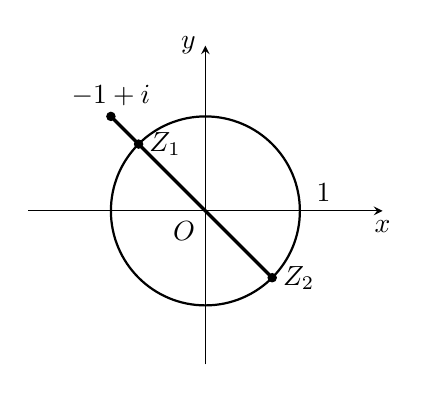
\begin{tikzpicture}[>=stealth, scale=1.5]
\draw[->](-1.5,0)--(1.5,0)node[below]{$x$};
\draw[->](0,-1.3)--(0,1.4)node[left]{$y$};
\draw[thick](0,0)node[below left]{$O$}circle(.8);
\draw[very thick](-45:.8)node[right]{$Z_2$}--(90+45:.8)node[right]{$Z_1$}--(-.8,.8)node[above]{$-1+i$};
\node at (1,0)[above]{$1$};
\draw[fill](-45:.8) circle(1pt);
\draw[fill](180-45:.8) circle(1pt);
\draw[fill](-.8,.8) circle(1pt);

\end{tikzpicture}
\captionof{figure}{}
\end{minipage}

\textbf{解5:}(利用$|z|^2=z\cdot \bar z$)考虑
\[|z+1-i|^2=(z+1-i)\cdot \overline{(z+1-i)}\]

$\because\quad z=\cos\theta+i\sin\theta$,代入上式有
\[\begin{split}
|z+1-i|&=[(1+\cos\theta)+(-1+\sin\theta)i][(1+\cos\theta)-(-1+\sin\theta)i]\\
&=(1+\cos\theta)^2+(1-\sin\theta)^2\\
&=3+2(\cos\theta-\sin\theta)    
\end{split}\]
(以下同解1)
\end{solution}

\begin{rmk}
    解法1与2是利用模的定义,解法3、5是利用模的性质,解法4是利用模的几何意义,解法5则别开生面。
\end{rmk}

\begin{example}
    若$|z|=1$,当$z$为何值时,$|z^2-z+1|$能取到最大(小)值。
\end{example}

\begin{solution}
由$|z|=1$知$z\cdot \bar z=1$.

设$z=a+bi\; a,b\in\R$
\[\begin{split}
    |z^2-z+1|=|z^2-z+1|\cdot |\bar z|&=|z^2\cdot \bar z-z\cdot \bar z+\bar z|\\
    &=|z-1+\bar z|=|2a-1|
\end{split}\]

$\because\quad |z|=1\Rightarrow -1\le a\le 1$

$\therefore\quad |2a-1|_{\max}=|2(-1)-1|=3$(当$z=-1$时);$|2a-1|_{\min}=0$(当$z=\frac{1}{2}\pm\frac{\sqrt{3}}{2}i$时).
\end{solution}

\begin{rmk}
    这里以$|z|$乘$|z^2-z+1|$为的是使其“降次”化简(还可以用$1=z\cdot \bar z$代入达到降次的目的)。
\end{rmk}

\begin{example}
    已知$z_1,z_2\in\mathbb{C}$,且$|z_1-\bar z_2|=|1-z_1z_2|$,

求证:$|z_1|$与$|z_2|$中至少有一个等于1.\hfill (*)
\end{example}

\begin{analyze}
    欲证(*),应证$(|z_1|-1)(|z_2|-1)=0$. 因而由条件应设法分解因式。
\end{analyze}

\begin{proof}
\[\begin{split}
    |z_1-\bar z_2|&=|1-z_1z_2|\\
     |z_1-\bar z_2|^2&=|1-z_1z_2|^2\\
(z_1-\bar z_2)\overline{(z_1-\bar z_2)}&=(1-z_1z_2)\overline{(1-z_1\cdot z_2)}   \\
 (z_1-\bar z_2)(\bar z_1-z_2)&=(1-z_1z_2)(1-\bar z_1\cdot \bar z_2)     \\
     |z_1|^2-z_1z_2-\bar z_1\bar z_2 +|z_2|^2&=1-\bar z_1\bar z_2-z_1z_2+|z_1|^2\cdot |z_2|^2     
\end{split}\]

$\therefore\quad |z_1|^2\cdot |z_2|^2-|z_1|^2- |z_2|^2+1=0 \Rightarrow (|z_1|^2-1)(|z_2|^2-1)=0$

因此:$|z_1|^2=1$或$|z_2|^2=1$,即
\[|z_1|=1\quad\text{或}\quad |z_2|=1\]
\end{proof}

\begin{rmk}
    这里解题目标的确立对思路起了“导航”作用。
\end{rmk}

\begin{example}
    求满足$|z+3-\sqrt{3}i|\le \sqrt{3}$,且有最小辐角的复数$z$。
\end{example}

\begin{solution}
    满足$|z+3-\sqrt{3}i|\le \sqrt{3}$,即
$\left|z-(-3+\sqrt{3}i)\right|\le \sqrt{3}$的点$z$分布在以点$z_0=-3+\sqrt{3}i$为圆心,以$\sqrt{3}$为半径的包括边界的圆面上。很明显,过原点$O$引圆的另一条切线$OZ_1$(图6.29),则切点$Z_1$对应的复数的辐角比圆面上其他任何点对应的复数的辐角都要小。因此,只要求出复数$z_1$来就行了.

\noindent
\begin{minipage}{.55\textwidth}
\CTEXindent  连接$OZ_0,AZ_0,Z_0Z_1$,据平面几何知识知道,
$|OA|=|OZ_1|=3$,且$\angle 1=\angle 2$,而$\angle 1=\frac{\pi}{6}$

$\therefore\quad \arg z_1=\pi-2\angle 1=\frac{2\pi}{3}$,从而
\[z_1=3\left(\pc{\frac{2\pi}{3}}\right)=-\frac{3}{2}+\frac{3\sqrt{3}}{2}i\]
$\therefore\quad z=-\frac{3}{2}+\frac{3\sqrt{3}}{2}i$    
\end{minipage}\hfill
\begin{minipage}{.4\textwidth}
\centering
\begin{tikzpicture}[>=stealth, scale=.8]
\draw[->](-5,0)--(1,0)node[below]{$x$};
\draw[->](0,-1.5)--(0,4.5)node[left]{$y$};
\draw(-3,1.732)circle(1.732);
\tkzDefPoints{-3/0/A, 0/0/O, -3/1.732/Z_0}
\tkzDefPoint(120:3){Z_1}
\tkzLabelPoints[left](Z_0)
\tkzLabelPoints[below](A)
\tkzLabelPoints[above](Z_1)
\tkzLabelPoints[below left](O)
\tkzDrawSegments(O,Z_1)
\tkzDrawSegments[dashed](O,Z_0 Z_0,Z_1 A,Z_0)
\tkzMarkRightAngles[size=.2](Z_0,A,O Z_0,Z_1,O)
\tkzMarkAngles[mark=none, size=.75](Z_1,O,Z_0)
\tkzMarkAngles[mark=none, size=.65](Z_0,O,A)
\tkzLabelAngle[pos=1](Z_0,O,A){1}
\tkzLabelAngle[pos=1](Z_1,O,Z_0){2}
\end{tikzpicture}
\captionof{figure}{}
\end{minipage}
\end{solution}

\begin{rmk}
    充分利用复数的几何意义,采用数形结合的方法,是解决复数问题的重要途径。
\end{rmk}

\begin{example}
设$z_1,z_2\in\mathbb{C}$,满足$z_1\cdot \bar z_2+\bar A\cdot z_1+A\cdot \bar z_2=0$,$A$是不为零的复数。求证:
\begin{enumerate}
    \item $|z_1+A|\cdot |z_2+A|=|A|^2$
    \item $\frac{z_1+A}{z_2+A}=\left|\frac{z_1+A}{z_2+A}\right|$
\end{enumerate}
\end{example}

\begin{analyze}
    处理附条件等式证明题的基本方法是推出法和代入法。

我们先看看推出法。欲证明(1)式,联系到已知,只要推出下式即可。
\begin{equation}
    (z_1+A)\overline{(z_2+A)}=A^2 \tag{*}
\end{equation}

这是把条件式分解因式的结果(先确立解题目标,为思路“导航”).

若使用代入法,既可由已知解出$z_1$代入(留给读者试试)。也可以把条件式“代入”,为此,先把(1)式左边变形。
\end{analyze}

\begin{proof}
    \textbf{证法1:}由$z_1\cdot \bar z_2+\bar A\cdot z_1+A\cdot \bar z_2=0$(注意其结构特征)
得
\[(z_1+A)(\bar z_2+\bar A)=A\bar A=|A|^2\]
对此式两边取模,得
\[|(z_1+A)\overline{(z_2+A)}|=|A|^2\]
即
\[|z_1+A|\cdot |z_2+A|=|A|^2\]

\textbf{证法2:}
\[\begin{split}
    |z_1+A|\cdot |z_2+A|&=|z_1+A|\cdot |\bar z_2+\bar A|\\
&=|(z_1+A)(\bar z_2+\bar A)|=|z_1\bar z_2+z_1\bar A+A\bar z_2+A\bar A|\\
\text{代入条件} \to &=|0+A\bar A|=|A|^2
\end{split}\]

现在来证明(2):由左$\Rightarrow$右,(由左式先构造出右边的分母)
\[\begin{split}
\frac{z_1+A}{z_2+A}&=\frac{(z_1+A)\overline{(z_2+A)}}{(z_2+A)\overline{(z_2+A)}}\\
&=\frac{z_1\bar z_2+A\bar z_2+A\bar z_1+A\bar A}{|z_2+A|^2}\\
\text{代入条件} \to &=\frac{|A|^2}{|z_2+A|^2}=\frac{|z_1+A|\cdot |z_2+A|}{|z_2+A|^2}=\left|\frac{z_1+A}{z_2+A}\right|
\end{split}\]
(2)的证明有多种思路,读者可以自己试试.
\end{proof}

\section*{习题十二}
\begin{center}
    \bfseries A
\end{center}

\begin{enumerate}
    \item 若$z\in\mathbb{C}$,求证$z+\frac{1}{z}$为实数的充要条件是$|z|=1$.
    \item   若$|z+2i|\le 1$, 求$|z|$的最大(小)值。
    \item   若$|z|=3$,求$|z-3i|$的最大值。
    \item   若$|z|=1$,求证$\left|\frac{z-z_0}{1-z\bar z_0}\right|=1$(用多种方法)。
    \item   复数$z$满足$|z-4i|\le 2$,则$\arg z$的最大值是\blank,最小值是\blank.
\end{enumerate}

\begin{center}
    \bfseries B
\end{center}

\begin{enumerate}\setcounter{enumi}{5}
    \item 若$z\cdot \bar z+(1-2i)z+(1+2i)\bar z\le 3$。求$|z|$的最大(小)值。
\item 复数$z$满足$2|z-3-3i|=|z|$,求$|z|$的最大(小)值。
\item 若$a,b,c,d\in\R$, 且$a+b=8$, $c+d=12$,求$(a+bi)$, $(c+di)$的模的最小值。
\item 设$z_1=\sqrt{a-5}+ai\; (a\ge 5,\; a\in\R)$,$z_2=2\cos\theta+3i\sin\theta,\; \theta\in\R$. 求$(z_1-z_2)(\bar z_1-\bar z_2)$的最小值。
\item 若$z+\frac{4}{z}\in\R$,且$|z-2|=2$,求复数$z$。
\item 若$k\in\R$, $z=\cos\theta+i\sin\theta$,
\begin{enumerate}[(1)]
\item $k$与$\theta$各为何值时,$z^3+k\bar z^3$为纯虚数;
\item 若$k>0$,当$\theta$变化时,求$|z^3+k\bar z^3|$的最大(小)值。
\end{enumerate}

    \item 设$z=1+\sin\alpha+i\cos\alpha\; \left(-\pi<\alpha<-\frac{\pi}{2}\right)$,求$|z|$与$\arg z$.
    \item 设$z=\pc{\theta}\; (\pi<\theta<2\pi)$,求$z^2+z$的模与辐角。
\end{enumerate}


\subsection{复数与几何}

\begin{example}
求点$z$的轨迹($t$为参数,且$t\in\R$)
\begin{multicols}{3}
\begin{enumerate}[(1)]
    \item $z=t(1+i)$
    \item $z=t+\frac{i}{t}$
    \item $z=a\cos t+ib\sin t$
\end{enumerate}
\end{multicols}
\end{example}

\begin{solution}
\begin{enumerate}[(1)]
    \item $\because\quad z=t+it$,令$z=x+yi\; (x,y\in\R)$,则
\[\begin{cases}
    x=t\\y=t
\end{cases}\]
消去$t$,得$x=y$.

$\therefore\quad $点$z$的轨迹是第I、III象限的角平分线.

\item $z=t+\frac{i}{t}$,令$z=x+yi\; (x,y\in\R)$,则
\[\begin{cases}
    x=t\\[1.5ex] y=\frac{1}{t}
\end{cases}\]
消去$t$,得轨迹方程$xy=1$.

$\therefore\quad $轨迹为等轴双曲线$xy=1$.

\item $z=a\cos t+ib\sin t$,令$z=x+yi\; (x,y\in\R)$,得
\[\begin{cases}
x=a\cos t\\y=b\sin t
\end{cases}\]
由此得$\left(\frac{x}{a}\right)^2+\left(\frac{y}{b}\right)^2=1$

$\therefore\quad $轨迹是在标准位置上的椭圆.
\end{enumerate}
\end{solution}    

\begin{rmk}
对这类轨迹问题,我们设$z=x+yi\; (x,y\in\R)$,正确地实现$z$的实、虚部分离即可.
\end{rmk}


\begin{example}
点$F$为椭圆$\frac{x^2}{4}+y^2=1$的右焦点,$A$为椭圆上的动
点,$FABC$是正方形(图6.30),当$A$在椭圆上运动一圈时,求点$C$的轨迹。
\end{example}

\begin{solution}
设$C$点表示的复数为$x+yi$,$A$点表示的复数为$a+bi\; (x,y,a,b\in\R)$,

$\because\quad z_{\vv{OF}}=\sqrt{3},\quad z_{\vv{OC}}=x+yi$

$\therefore\quad z_{\vv{FC}}=z_{\vv{OC}}-z_{\vv{OF}}=x-\sqrt{3}+yi$

$\because\quad FABC$是正方形,

$\therefore\quad z_{\vv{FA}}=z_{\vv{FC}}\cdot i=-y+\left(x-\sqrt{3}\right)i$

而$z_{\vv{OA}}=z_{\vv{OF}}+z_{\vv{FA}}=\sqrt{3}-y+\left(x-\sqrt{3}\right)i$,
又$z_{\vv{OA}}=a+bi$

\noindent
\begin{minipage}{.55\textwidth}\CTEXindent
$\therefore\quad \begin{cases}
    a=\sqrt{3}-y\\
    b=x-\sqrt{3}
\end{cases}$

$\because\quad $点$A$在椭圆$\frac{x^2}{4}+y^2=1$上运动

$\therefore\quad \frac{\left(\sqrt{3}-y\right)^2}{4}+\left(x-\sqrt{3}\right)^2=1$,即    
\[\left(x-\sqrt{3}\right)^2+\frac{\left(y-\sqrt{3}\right)^2}{4}=1\]
\end{minipage}\hfill
\begin{minipage}{.4\textwidth}
\centering
\begin{tikzpicture}[>=stealth, scale=.8]
\draw[->](-3,0)--(3,0)node[below]{$x$};
\draw[->](0,-2)--(0,2)node[left]{$y$};
\node [below left]{$O$};
\draw(0,0)ellipse(2 and 1);
\tkzDefPoints{.866/0/F, .25/.992/A}
\tkzDefPointBy[rotation=center F angle -90](A)  \tkzGetPoint{C}
\draw[->, thick](F)node[below]{$F$}--(A)node[above]{$A$};
\draw[->,  thick](F)--(C)node[right]{$C$};
\tkzDefPointBy[translation=from F to A](C)   \tkzGetPoint{B}
\tkzDrawSegments(A,B B,C)
\tkzLabelPoints[above](B)

\end{tikzpicture}
\captionof{figure}{}
\end{minipage}

$\therefore\quad C$点的轨迹是长轴垂直于$Ox$轴且交于$F$点的竖立的椭圆。
\end{solution}

\begin{example}
    若$\delta =\omega i+3$,复数$\omega$对应的点在曲线
\begin{equation}
    |z-5|-|z+5|=6 \tag{1}
\end{equation}
上运动,在复平面上求出复数$\delta$对应的点的轨迹方程,并画出图形。
\end{example}

\begin{analyze}
\textbf{分析1:}
(1)是双曲线的左半支,$\omega$对应的点在其上运动,利用(1)的参数方程可以写出$\omega$,从而可得出$\delta$的表达式,使问题获解。

\textbf{分析2:}  由于$\omega$对应的点$A$在(1)上运动,有
\begin{equation}
    |\omega -5|-|\omega+5|=6\tag{2}
\end{equation}
利用$\delta=\omega i+3$,可由(2)直接通过代换,得出$\delta$对应的点$B$所满足的方程。

\textbf{分析3:}
由于$\omega$ 对应的点$A$在已知曲线$C$上运动,$\delta =\omega i+3$, 根据复数乘法与加法的意义,也可以利用几何方法处理之。
\end{analyze}

\begin{solution}
   \textbf{解1:}由(1)可得$a=3,\; c=5,\; b=4$, 而可把(1)写成普通方程: 
\[\frac{x^2}{9}-\frac{y^2}{16}=1,\quad (x<0)\]

$\therefore\quad \begin{cases}
    x=3\sec\theta \\ y=4\tan\theta
\end{cases} \Rightarrow \omega =3\sec\theta+i4\tan\theta,\quad \left[\theta\in\left(\frac{\pi}{2},\frac{3\pi}{2}\right)\right]$

令$\delta=x+yi\; (x,y\in\R)$

$\therefore\quad \begin{cases}
    x=3-4\tan\theta  \\ y=3\sec\theta 
\end{cases},\quad \theta\in\left(\frac{\pi}{2},\frac{3\pi}{2}\right)$

消去参数$\theta$,可得
\[-\frac{(x-3)^2}{4}+\frac{y^2}{9}=1,\quad (y<0)\]
画出其图形(图6.31)

\noindent
\begin{minipage}{.55\textwidth}\CTEXindent
\textbf{解2:}由$\delta =\omega i+3$得$\omega =3i-\delta i$,代入(2)得
\[|-\delta i+3i-5|-|-\delta i+3i+5|=6\]
两边同乘$|i|$,得
\[|\delta -5i-3|-|\delta +5i-3|=6\]
而
$|\delta -(3+5i)|-|\delta -(3-5i)|=6$,
其轨迹是以$(3+5i)$, $(3-5i)$为焦点,$2a=6$的双曲线的下半支(图6.31)。    
\end{minipage}
\begin{minipage}{.4\textwidth}
\centering
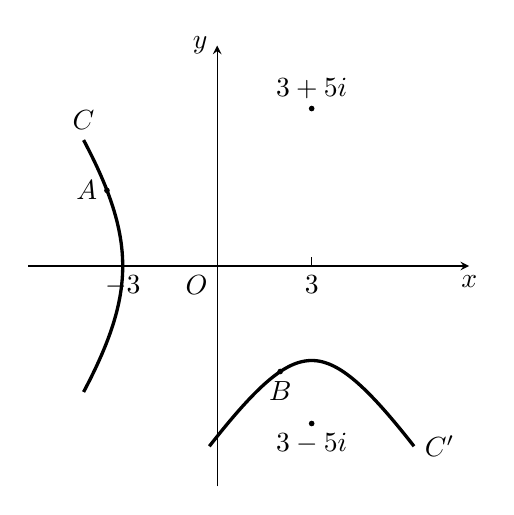
\begin{tikzpicture}[>=stealth, scale=.4]
    \draw[->](-6,0)--(8,0)node[below]{$x$};
    \draw[->](0,-7)--(0,7)node[left]{$y$};
\draw[domain=-4:4, samples=100, smooth, very thick]plot({-sqrt(9+9/16*\x*\x)}, \x)node[above]{$C$};
\foreach \x in {3,-3}
{
    \draw(\x,0)node[below]{$\x$}--(\x,.3);
}
\node[below left]{$O$};
\draw[fill](3,-5)node[below]{$3-5i$}  circle (2pt);
\draw[fill](3,5)node[above]{$3+5i$}  circle (2pt);
\draw[fill](-3.5,2.4)node[left]{$A$}  circle (2pt);

\draw[domain=-3.25:3.25, samples=100, smooth, very thick]plot(\x+3, {-sqrt(9+2.25*\x*\x)})node[right]{$C'$};
\draw[fill](2,-3.35)node[below]{$B$}  circle (2pt);
% \draw[fill](.6,-3.5)node[below]{$B$}  circle (2pt);

\end{tikzpicture}
\captionof{figure}{}
\end{minipage}


\textbf{解3:}由于$\omega$ 对应的点$A$在曲线$C$上运动,$\delta =\omega i+3$,从而把曲线$C$绕原点逆时针旋转$\frac{\pi}{2}$,再向右平移3个单位,便
得到$\delta $对应的点$B$的轨迹$C'$(图6.31).此时,曲线$C$的焦点$\pm 5$变成$\pm 5i+3$,也就是$3\pm 5i$. 由于旋转中,曲线的形状、大小均不变,所以$2a=6$,由此,曲线$C'$的方程应为
\[|\delta -(3+5i)|-|\delta -(3-5i)|=6\]
\end{solution}


\begin{example}
    若$\frac{z}{z-1}$为纯虚数,求点$x$的轨迹.
\end{example}

\begin{solution}
\textbf{解1:}设$\frac{z}{z-i}=bi\; (b\in\R,\; b\ne 0)$,则$(1-bi)z=-bi$. 由于$1-bi\ne 0$,

$\therefore\quad z=\frac{-bi}{1-bi}=\frac{b^2-bi}{1+b^2}$

令$z=x+yi\; (x,y\in\R)$,得
\[\begin{cases}
x=\frac{b^2}{1+b^2}
\\[1.5ex]
y=\frac{-b}{1+b^2}
\end{cases}(b\ne 0) \xrightarrow[]{\text{消参}}x^2+y^2=x\; (xy\ne 0)\Rightarrow \left(x-\frac{1}{2}\right)^2+y^2=\frac{1}{4}\; (xy\ne 0) \]
这是以$\left(\frac{1}{2},0\right)$为圆心,以$\frac{1}{2}$为半径的圆[除去$(0,0)$、$(1,0)$点].

\textbf{解2:}
$\because\quad \frac{z}{z-1}$为纯虚数

\[\begin{split}
    \therefore\quad \overline{\left(\frac{z}{z-1}\right)}&=-\left(\frac{z}{z-1}\right)\quad (z\ne 0)\\
    \frac{\bar z}{\overline{z-1}}+\frac{z}{z-1}&=0\\
    \frac{2|z|^2-(z+\bar z)}{|z-1|^2}&=0  \quad (z\ne 0)
\end{split}\]
设$z=x+yi\; (x,y\in\R)$,由上式得
\[2(x^2+y^2)-2x=0\Rightarrow \left(x-\frac{1}{2}\right)^2+y^2=\frac{1}{4}\; (xy\ne 0)\]
(以下略).

\textbf{解3:}
设$z=x+yi\; (x,y\in\R)$
\[\frac{z}{z-1}=\frac{x+yi}{x-1+yi}=\frac{x^2+y^2-x-yi}{(x-1)^2+y^2}\]

$\because\quad \frac{z}{z-1}$是纯虚数

$\therefore\quad \begin{cases}
    (x-1)^2+y^2\ne 0\\
    x^2+y^2-x=0\\
    -y\ne 0
\end{cases}$
即$\left(x-\frac{1}{2}\right)^2+y^2=\frac{1}{4}\; (y\ne 0)$(以下略).
\end{solution}

\section*{习题十三}
\begin{center}
    \bfseries A
\end{center}
\begin{enumerate}
    \item 已知定点$A(1,0)$和动点$B(0,t),\; t\in\R$. 若$ABC$是等边三角形($A$,$B$,$C$是顺时针方向标注)。试求点$C$的轨迹。
    \item 点$B$在单位圆上运动,$\vv{OA}=2$, $\triangle ABC$是正三角形($A$、$B$、$C$顺时针方向标注),求点$C$的轨迹方程。
    \item 设复数$\omega$对应的点在单位圆上运动,
    设$\delta =\omega-\frac{1}{\omega}$,求$\delta$对应的点的轨迹。
   \item 已知复平面内一点$z$到$(-5,0)$与$(5,0)$的距离之差为6,
   \begin{enumerate}[(1)]
   \item 写出点$z$满足的复数方程,并画出图形;
   \item 若点$P$在上述曲线上运动,求等边三角形$OPQ$顶点$Q$的轨迹方程($O$,$P$,$Q$为逆时针方向标注)。
   \end{enumerate}
\end{enumerate}


\begin{center}
    \bfseries B
\end{center}

\begin{enumerate}\setcounter{enumi}{4}
    \item 若点$B$在半圆$x^2+y^2=1\; (-1\le x\le 1,\; 0\le y\le 1)$上运动,点$A$为$(2,0)$,且$\triangle ABC$是以$BC$为斜边的等腰直角三角形。问点$B$在何处时,点$O$到点$C$的距离最长,并求这个最长的距离。
    \item 若复数$z$满足
    $(z-3)(\bar z-3)+(z+3)(\bar z+3)=2(|z^2-9|+2)$.
    求点$z$表示的图形,并求出它的普通方程。
    \item 若$z_1=-1+i$, $z_2=1+i$, 复数$z$对应的点在线段$z_1z_2$上运动,求$z^2$对应的点的轨迹的普通方程。
    \item 已知$z\cdot \bar z-\bar A\cdot z-A\cdot \bar z=0$,其中$z,A\in\mathbb{C}$,且$A$为常数,求复数$z$表示的点的轨迹。
\end{enumerate}

\subsection{其他几何问题}
    复数及其计算有明确的几何意义。因此,复数与几何有天然的联系,除了上述轨迹问题以外,再看几个例子。

\noindent
\begin{minipage}{.55\textwidth}
    \CTEXindent
\begin{example}
    三个互不相等的复数$z_1$,$z_2$,$z_3$满足
$z_1+z_2+z_3=0$, 且$|z_1|=|z_2|=|z_3|$,这三个复数在复平面上的对应点为$A,B,C$,

求证:$\triangle BAC$是正三角形(图6.32).
\end{example}    
\end{minipage}\hfill
\begin{minipage}{.4\textwidth}
\centering
\begin{tikzpicture}[>=stealth]
    \draw[->](-2,0)--(2,0)node[below]{$x$};
    \draw[->](0,-1.5)--(0,1.5)node[left]{$y$};
\draw(0,0)node[below right]{$O$} circle(1); 
\tkzDefPoint(70:1){A}
\tkzDefPoint(70+120:1){B}
\tkzDefPoint(70+240:1){C}
\tkzDefPoint(0,0){O}
\tkzDrawPolygon(A,B,C)
\tkzInterLL(B,C)(A,O) \tkzGetPoint{D}
\draw[dashed](A)--(D);
\node at (A)[above right] {$A(Z_1)$};
\node at (B)[below left]{$B(Z_2)$};
\node at (C)[below right]{$C(Z_3)$};

\end{tikzpicture}
\captionof{figure}{}
\end{minipage}

\begin{proof}
\textbf{证明1:}
$|z_1|=|z_2|=|z_3|\Rightarrow $原点$O$是$\triangle ABC$的外心。

$z_1+z_2+z_3=0\Rightarrow $
原点是$\triangle ABC$的重心。

设$z_k=a_k+b_k i,\; k=1,2,3$,则由
\[\begin{split}
    z_1+z_2+z_3=0 &\Rightarrow (a_1+a_2+a_3)+(b_1+b_2+b_3)i=0\\
    &\Rightarrow \frac{a_1+a_2+a_3}{3}+\frac{b_1+b_2+b_3}{3}i=0\\
    &\Rightarrow \frac{a_1+a_2+a_3}{3}=0\quad \text{且}\quad \frac{b_1+b_2+b_3}{3}=0
\end{split}\]

$\therefore\quad \triangle ABC$的重心为$(0,0)$.

由于$\triangle ABC$的外心与重心重合,

$\therefore\quad \triangle ABC$是正三角形。

\begin{rmk}
    事实上可以证明了$\triangle ABC$的重心是$\frac{z_1+z_2+z_3}{3}$, 
这是一个重要的结论。
\end{rmk}

\noindent
\begin{minipage}{.55\textwidth}\CTEXindent
    \textbf{证明2:}反向延长$\vv{OZ_1}$,交圆于$Z_1'$,则$Z_1'=-Z_1$.

由$z_1+z_2+z_3=0\Rightarrow -z_1=z_2+z_3$

$\therefore\quad z_2+z_3=z_1'\Rightarrow OZ_2Z_1'Z_3$是平行四边形.
    
又由$|z_2|=|z_3|$知$OZ_2Z_1'Z_3$是菱形(图6.33).

由于$|z_1'|=|z_1|=|z_2|\Rightarrow \triangle OZ_2Z_1'$是正三角形.
从而$\angle Z_2OZ_3=120^{\circ}$. 

同理,
$\angle Z_3 OZ_1=\angle Z_1OZ_2=120^{\circ}$

$\therefore\quad \triangle Z_1Z_2Z_3$是正三角
形。
\end{minipage}
\hfill
\begin{minipage}{.4\textwidth}
\centering
\begin{tikzpicture}[>=stealth, scale=1.3]
    \draw[->](-1.8,0)--(1.8,0)node[below]{$x$};
    \draw[->](0,-1.5)--(0,2)node[left]{$y$};
\draw(0,0)node[below left]{$O$} circle(1); 
\tkzDefPoint(70:1){Z_1}
\tkzDefPoint(70+120:1){Z_2}
\tkzDefPoint(70+240:1){Z_3}
\tkzDefPoint(70+180:1){Z_1'}
\tkzDefPoint(0,0){O}
\tkzDrawPolygon(Z_1,Z_2,Z_3)
\tkzDrawSegments[dashed](Z_1',Z_2 Z_1',Z_3 Z_1,Z_1' O,Z_2 O,Z_3)
\tkzAutoLabelPoints[center=O, dist=.3](Z_1,Z_2,Z_3,Z_1')

\end{tikzpicture}
\captionof{figure}{}
\end{minipage}

\textbf{证明3:}也可以去证$|AB|=|AC|=|BC|$.\hfill (*)

\[\begin{split}
    \because\quad |AB|&=|z_1-z_2|,\quad |AC|=|z_1-z_3|\\
|z_1-\bar z_2|^2&=(z_1-z_2)\overline{(z_1-z_2)}=|z_1|^2+|z_2|^2-(z_1\bar z_2+\bar z_1z_2)\\
|\bar z_1-z_3|^2&=(z_1-z_3)\overline{(z_1-z_3)}=|z_1|^2+|z_3|^2-(z_1\bar z_3+\bar z_1z_3)    
\end{split}\]

$\because\quad |z_1|=|z_2|=|z_3|=r$

$\therefore\quad$欲证(*),只要证
\begin{equation}
 z_1\cdot \bar z_2+\bar z_1\cdot z_2=z_1\cdot \bar z_3+\bar z_1\cdot z_3=z_2\cdot \bar z_3+\bar z_2\cdot z_3 \tag{**} 
\end{equation}
这是一个轮换对称式,欲证它,只要证$z_1\cdot \bar z_2+\bar z_1\cdot z_2$是个常量。
\[\begin{split}
\begin{cases}
    -z_3=z_1+z_2\\
    -\bar z_3=\bar z_1+\bar z_2
\end{cases}&\Rightarrow |x_3|^2 =z_1\bar z_1+z_2\bar z_2+z_1 z_2+z_2\bar{\bar z_1}\\
&\Rightarrow |x_3|^2 =|z_1|^2+|z_2|^2+z_1 \bar z_2+\bar z_1 z_2\\
&\Rightarrow z_1 \bar z_2+\bar z_1 z_2=|x_3|^2-|z_1|^2-|z_2|^2=-|x_3|^2=-r^2
\end{split}\]

$\therefore\quad $(**)成立,从而(*)成立,所以$\triangle ABC$是正三角形。
\end{proof}

\begin{example}
 已知$z\in\mathbb{C}$,且$|z_1|=|z_2|=|z_1-z_2|=a\; (a\in\R^+)$,

 求$z^3_1+z^2_1\cdot \bar z_2+\bar z_1\cdot z^2_2+z^3_2$的值.
\end{example}

\begin{analyze}
由$|z_1|=|z_2|=|z_1-z_2|=a\; (a\in\R^+)$, 知$z_1,z_2$都是非零复数,且点$Z_1$,点$Z_2$与原点构成正三角形的三个顶点(这一点是解此题的突破口!)。 
\end{analyze}

\begin{solution}
设$z_2=z_1\left(\pc{\frac{\pi}{3}}\right)=z_1\left(\frac{1}{2}+\frac{\sqrt{3}}{2}i\right)$,代入原式:
\[\begin{split}
    &\qquad z^3_1+z^2_1\cdot \bar z_2+\bar z_1\cdot z^2_2+z^3_2\\
    &=z^3_1+z^2_1\cdot \bar z_1\overline{\left(\frac{1}{2}+\frac{\sqrt{3}}{2}i\right)}+\bar z_1\cdot z^2_1\left(\frac{1}{2}+\frac{\sqrt{3}}{2}i\right)^2+z^3_1\left(\frac{1}{2}+\frac{\sqrt{3}}{2}i\right)^3\\
    &=z^3_1+z_1\cdot |z_1|^2\left(\frac{1}{2}-\frac{\sqrt{3}}{2}i\right)+z_1\cdot |z_1|^2\left(-\frac{1}{2}+\frac{\sqrt{3}}{2}i\right)-z^3_1=0
\end{split}\]
\end{solution}

\section*{习题十四}
\begin{center}
    \bfseries A
\end{center}
\begin{enumerate}
    \item \begin{enumerate}[(1)]
    \item 设$\omega=-\frac{1}{2}+\frac{\sqrt{3}}{2}i$,复平面上有三个点:$O(0)$,
    $A(\omega-z)$, $B(\omega+z)$(括号内表示该点对应的复数),而且这三个点构成等腰直角三角形,$\angle AOB=\frac{\pi}{2}$,求$z$。
    \item $\arg(z+1)=\frac{\pi}{6}$, $\arg(z-1)=\frac{2\pi}{3}$,求$z$。
    \item 在复平面上,直角$\triangle ABC$的三个顶点$A$、$B$、$C$分别对应复数$z$、$z^2$、$z^3$,且$|z|=2$, $\angle BAC=90^{\circ}$,求$z$。
    \end{enumerate}

    \item 对于两个非零复数$z_1$,$z_2$,对应它们的向量分别是$\vv{OZ_1}$与$\vv{OZ_2}$,
    
    求证:$\vv{OZ_1}\bot\vv{OZ_2}\Leftrightarrow R(z_1\cdot \bar z_2)=0$.
\end{enumerate}
    
\begin{center}
    \bfseries B
\end{center}
\begin{enumerate}\setcounter{enumi}{2}
    \item 设$A=\{z\mid |z+1|\le |z-i|\}$,$B=\{z\mid |z+2|\le 2\}$, $C=A\cap B$,
    求点集$C$的图形占有的面积。
    \item $P$、$Q$是复平面上的点集:
\[\begin{split}
    P&=\{z\mid z\cdot \bar z+3i\bar z-3iz+5=0\},\\
    Q&=\{\delta |\delta =2iz,\; z\in P\}
\end{split}\]
\begin{enumerate}[(1)]
\item 点集$P$、$Q$各表示什么曲线?在同一个坐标系中画出$P$、$Q$各表示的曲线;
\item 设$z_1\in P$, $z_2\in Q$,求$|z_1-z_2|$的最大(小)值。
\end{enumerate}

    \item 设复数集合$M=\{z\mid |z-2+i|\le 2,\; z\in\mathbb{C}\}\cap\{z\mid |z-2-i|=|z-4+i|,\; z\in\mathbb{C}\}$
\begin{enumerate}[(1)]
\item 在复平面上作出表示$M$的图形,并说明图形的名称;
\item 求$\arg z\; (z\in M)$的范围;
\item 求$|z|\; (z\in M)$的范围。 
\end{enumerate}
\end{enumerate}


\section{本章小结}
\subsection{知识结构分析}
\subsubsection{复数及其有关概念}
\begin{enumerate}
    \item 虚数单位$i$及其幂的运算性质。
\[\begin{split}
&    i^{4n}=1,\quad i^{4n+1}=i,\quad i^{4n+2}=-1,\quad i^{4n+3}=-i,\\
& i^n+i^{n+1}+i^{n+2}+i^{n+3}=0\quad (n\in\Z)
\end{split} \]
\item 对虚数单位i还规定实数与它可以进行四则运算,且原有的加、乘运算律仍然成立,从而出现了形如$a+bi\; (a,b\in\R)$的数,称此种数为复数。
\item 复数系:
\begin{center}
    \begin{tikzpicture}[>=stealth]
\node(A) at (-1,0)[text width=2cm, align=center]{复数\\ ($a+bi$)};
\node(B1) at (2,1)[text width=2cm, align=center, left]{实数\\ ($b=0$)};
\node(B2) at (2,-1)[text width=2cm, align=center, left]{虚数\\ ($b\ne 0$)};
\node(C1) at (4,0)[text width=2cm, align=center, left]{纯虚数\\ ($a=0$)};
\node(C2) at (4,-2)[text width=2cm, align=center, left]{非纯虚数\\ ($a\ne 0$)};
\draw[decorate, decoration={brace, amplitude=6pt}](0,-1.25)--(0,1.25);
\draw[decorate, decoration={brace, amplitude=6pt}](2,-2.25)--(2,0.25);

    \end{tikzpicture}
\end{center}
\item 复数的表示形式:
\begin{itemize}
\item 复数的代数形式:$z=a+bi\; (a,b\in\R)$;
\item 复数的几何形式:复平面内的一点$Z(a,b)$或向量$\vv{OZ}$;
\item 复数的三角形式:$z=r(\pc{\theta})$.
\end{itemize}

复数的三种表示形式之间是可以互化的,除了实数零以外,它们彼此之间都是一一对应的,即
\begin{center}
\begin{tikzpicture}[>=stealth]
\node(A) at (0,0){复数$z=a+bi$};
\node(B) at (5,0){复数$z=r(\pc{\theta})$};
\node(C) at (0,-2){点$Z(a,b)$};
\node(D) at (5,-2){向量$\vv{OZ}$};
\draw[<->](A)--(B);
\draw[<->](A)--(C);
\draw[<->](D)--(B);
\draw[<->](C)--(D);
\end{tikzpicture}
\end{center}

由复数的三种表示形式可知:确定一个复数需要两个实数,即确定一个复数要且仅要两个独立的条件。
\item 复数相等的条件:
\begin{itemize}
    \item 代数形式:$z_1=a+bi,\quad z_2=c+di\; (a,b,c,d\in\R)$
\[z_1=z_2\Longleftrightarrow \begin{cases}
    a=c\\ b=d
\end{cases}\]
\item 三角形式:$z_1=r_1(\pc{\theta_1}),\quad z_2=r_2(\pc{\theta_2})$
\[z_1=z_2\Longleftrightarrow \begin{cases}
    r_1=r_2\\ \theta_1=\theta_2+2k\pi\; (k\in\Z)
\end{cases}\]
\item 几何形式:相等的复数表示复平面内的同一个点,反之,复平面内的一个点表示的两个复数相等。
\end{itemize}

相等的复数在复平面内表示的两个向量方向一致且长度相等,反之,复平面内的两个向量方向一致且长度相等,则它们表示的两个复数相等(向量的起点不一定在原点)。

\item 复数的模及其运算性质:

复数的模,即是表示复数的向量的长度,
\[\begin{split}
   |z|&=|a+bi| =\sqrt{a^2+b^2}\quad (a,b\in\R)\\
    |z_1\cdot z_2|& =|z_1|\cdot |z_2|,\quad |z^n|=|z|^n,\quad \left|\frac{z_1}{z_2}\right|=\frac{|z_1|}{|z_2|}\; (z_1\ne 0)\\
   \big| |z_1|-|z_2| \big|& \le |z_1\pm z_2|\le |z_1|+|z_2|
\end{split}\]
(想一想上述不等式中等号成立的条件)
\item 复数的辐角:
以$x$轴的正半轴为始边,以向量$\vv{OZ}$所在的射线(起点是原点)为终边的角$\theta$,叫做复数$z$的辐角。辐角的主值记为$\arg z$,且$0\le \arg z<2\pi$,因此,$\theta=\arg z+2k\pi\; (k\in\Z)$
\item 共轭复数及其运算性质:
复数$z=a+bi\; (a,b\in\R)$的共轭复数记为$\bar z=a-bi$.
\[\begin{split}
    \overline{z_1\pm z_2}=\bar z_1\pm\bar z_2,&\qquad \overline{z_1\cdot z_2}=\bar z_1\cdot \bar z_2\\
    \overline{\left(\frac{z_1}{z_2}\right)}=\frac{\bar z_1}{\bar z_2}\; (z_2\ne 0),&\qquad |z|^2=z\cdot \bar z=a^2+b^2
\end{split}\]
\end{enumerate}

\subsubsection{复数的运算及其几何意义}

\[\begin{split}
    \vv{OZ}: \; z&=a+bi=r(\pc{\theta});\\
    \vv{OZ_1}: \; z_1&=a_1+b_1i=r_1(\pc{\theta_1});\\
    \vv{OZ_2}: \; z_2&=a_2+b_2i=r_2(\pc{\theta_2});\\
\end{split}\]

\begin{enumerate}
    \item 复数的加减法
\[z_1\pm z_2=(a+1+b_1i)\pm (a_2+b_2i)=(a_1\pm a_2)+(b_1\pm b_2)i\]

复数的加、减法运算通常用复数的代数形式进行,其几何意义可用平行四边形法则或三角形法则确定。
\item 复数的乘法:
\[\begin{split}
    z_1\cdot z_2&=(a_1+b_1i)(a_2+b_2i)\\&=(a_1a_2-b_1b_2)+(a_1b_2+a_2b_1)i\\
    z_1\cdot z_2&=r_1(\pc{\theta_1})\cdot r_2(\pc{\theta_2})\\&=r_1r_2[\pcx{\theta_1+\theta_2}]
\end{split}
\]

积所对应的向量由$\vv{OZ_1}$,绕原点逆时针方向旋转$\theta_2$角,模伸长到原来的$r_2$倍来确定。
\item 复数的除法:
\[\begin{split}
    \frac{z_1}{z_2}&=\frac{a_1+b_1i}{a_2+b_2i}=\frac{a_1a_2+b_1b_2}{a^2_2+b^2_2}+\frac{a_2b_1-a_1b_2}{a^2_2+b^2_2}i\\
    \frac{z_1}{z_2}&=\frac{r_1(\pc{\theta_1})}{r_2(\pc{\theta_2}}=\frac{r_1}{r_2}[\pcx{\theta_1-\theta_2}]
\end{split}\]

商所对应的向量由$\vv{OZ_1}$绕原点顺时针方向旋转$\theta_2$角,模缩小到原来的$r_2$分之一来确定。商的几何意义经常用来确定向量$\vv{OZ_1}$与$\vv{OZ_2}$的夹角。
\item 复数的乘方:
\[\begin{split}
    z^n&=(a+bi)^n \quad \text{利用乘法公式运算}    \\
    z^n&=[r(\pc{\theta})]^n=r^n(\pc{n\theta})
\end{split}\]

幂所对应的向量由$\vv{OZ}$绕原点逆时针方向旋转$(n-1)\theta$角,模伸长到原来的$r^{n-1}$倍来确定。
\item 复数的开方:

$z=a+bi$的二次方根可根据方根的定义及复数相等的条件,利用代数的方法求得。

$z=r(\pc{\theta})$的$n$次方根为:
\[\sqrt[n]{r}\left[\pcx{\frac{\theta}{n}+\frac{2\pi}{n}k}\right]\quad (k=0,1,\ldots, n-1)\]

$n$次方根所对应的向量有且仅有$n$个,其模均为$\sqrt[n]{r}$,辐角组成$n$项等差数列,其首项为$\frac{\theta}{n}$,公差为$\frac{2\pi}{n}$,因此,复数开$n$次方所得到的$n$个$n$次方根所表示的点,均匀分布在以原点为圆心,以$\sqrt[n]{r}$为半径的圆上,组成一个正$n$边形。
\end{enumerate}


\subsection{本章应着重掌握的数学思想}
数形结合的思想应是本章的核心,它可以把十分抽象且缺乏实际意义的复数“几何化”,从而为复数在数学、物理技术上的应用开辟了道路。


\section*{复习题六}

\begin{center}
    \bfseries A
\end{center}

\begin{enumerate}
    \item 计算:
\begin{multicols}{2}
\begin{enumerate}[(1)]
    \item $i^{100}+i^{101}+i^{102}+\cdots +i^{1000}$
    \item $i+2i^2+3i^3+\cdots+100i^{100}$
    \item $\left(\frac{1+i}{1-i}\right)^{2n}$
    \item $i\cdot i^3\cdot i^5\cdots i^{99}$
\end{enumerate}
\end{multicols}

\item 判断下列命题的真假:
\begin{enumerate}[(1)]
\item 纯虚数与虚轴上的点是一一对应的;
\item 若$|z|=1$,则$-1\le z\le 1$;
\item $|z|^2=z^2$;
\item $z_1\cdot z_2=0$, 则$z_1,z_2$中至少有一个为零;
\item $z_1^2+z_2^2=0$,则$z_1=z_2=0$;
\item $|z_1|+|z_2|=0$,则$z_1=z_2=0$;
\item $i^n+i^{n+1}+i^{n+2}+i^{n+3}=0\quad (n\in\N)$.
\end{enumerate}

\item 已知复数$z=x+yi\; (x,y\in\R)$,求下列各式的实部与虚部:
\begin{multicols}{3}
\begin{enumerate}[(1)]
    \item $z^2$
    \item $z^3$
    \item $\frac{1}{z}$
\end{enumerate}
\end{multicols}

\item 求证: 
\begin{enumerate}[(1)]
    \item $(1+i)\left(1+\sqrt{3}i\right)(\pc{\theta})=2\sqrt{2}\left[\pcx{\frac{7\pi}{12}+\theta}\right]$
    \item $\frac{(1-\sqrt{3}i)(\pc{\theta})}{(1-i)(\cos\theta-i \sin\theta)}=\sqrt{2}\left[\pcx{2\theta-\frac{\pi}{12}}\right]$
\end{enumerate}

\item 化简
\[\frac{(\cos2\theta-i\sin2\theta)(\pc{\phi})^2}{\pcx{\theta+\phi}}\x \frac{(\pc{2\theta})^2(\cos2\phi-i\sin2\phi)}{\pcx{\theta-\phi}}\]
\item 设点$Z$表示复数$z$,在复平面内如何通过画图的方法,找出表示下列复数的点?
\begin{multicols}{2}
\begin{enumerate}[(1)]
    \item $z+(3+4i)$
    \item $z-4+i$
    \item $-\sqrt{2}z$
    \item $z(\pc{60^{\circ}})$
    \item $-iz$
    \item $\frac{a^2}{z}\; (a\in\R^+)$
\end{enumerate}
\end{multicols}

\item 当$\left(\frac{\sqrt{3}}{\frac{\sqrt{3}}{2}+\frac{\sqrt{3}}{2}i}\right)^n$为实数时,求$n$的最小正整数值.
\item $\vv{OZ}$表示复数$-1+i$,把$\vv{OZ}$逆时针旋转$120^{\circ}$,并拉长为原来的$\sqrt{3}$倍得到$\vv{OZ_1}$,设$\vv{OZ_1}$表示的复数是$z_1$,则$\bar z_1=\blank\blank$.

\item 设$z=\frac{1-\sin\theta+i\cos\theta}{1-\sin\theta-i\cos\theta}$
\begin{enumerate}[(1)]
    \item 当$\theta=\frac{\pi}{6}$时,计算$z$
    \item 若$0<\theta<\frac{\pi}{2}$,求$|z|$与$\arg z$
    \item 当$\theta=\frac{\pi}{5}$时,求使$z^n\in\R$的最小自然数$n$,并求此时$z^n$的值.
\end{enumerate}

\end{enumerate}

\begin{center}
    \bfseries B
\end{center}


\begin{enumerate}\setcounter{enumi}{9}
    \item 设$\alpha$,$\beta$是实系数一元二次方程的两个虚根。若$\frac{\alpha^2}{\beta}\in\R$, 求$\frac{\alpha}{\beta}$的值。
    \item 设$\alpha$,$\beta$分别是复平面上点$A$、$B$表示的复数。若$\alpha^2+\beta^2=\alpha\beta$, $\alpha\ne 0$且$|AB|=2$,
\begin{enumerate}[(1)]
    \item 求$\frac{\beta}{\alpha}$的辐角的主值与$|\alpha|$,
    \item 求向量$\vv{OA}+\vv{OB}$的模。
\end{enumerate}

    \item 关于$x$的二次方程$x^2+(2+i)x+4ab+(2a-b)i=0\; (a,b\in\R)$有实根,求点$P(a,b)$的轨迹$C$的方程,若曲线$C$是二次曲线,求其中心坐标和准线方程;若曲线$C$不是二次曲线,请说明理由。
    \item 若$z_A$,$z_B$是复平面上定点$A$,$B$表示的复数,设$z_P$是这个平面上动点$P$表示的复数,且
\[z_P=\frac{1-it}{2}\cdot z_A+\frac{1+it}{2}\cdot z_B\quad (t\in\R)\]
求点$P$的轨迹.

\item \begin{enumerate}[(1)]
    \item 证明:对于任意实数$t$,复数$z=\sqrt{|\cos t|}+\sqrt{|\sin t|}i$的模$r=|z|$适合$r\le \sqrt[4]{2}$.
    \item 当实数$t$取什么值时,复数$z=\sqrt{|\cos t|}+\sqrt{|\sin t|}i$的辐角的主值$\theta$满足$0\le \theta\le \frac{\pi}{4}$.
\end{enumerate}

\item 设$z_1$,$z_2$是复平面上两动点,$O$为原点,且满足:
\begin{enumerate}[(1)]
\item $z_1,z_2$表示的复数的辐角分别是$\theta,-\theta\; (0<\theta<90^{\circ})$;
\item $\triangle Z_1OZ_2$的面积为定值$S$;
\end{enumerate}
求$\triangle Z_1OZ_2$的重心$Z$表示的复数$z$的模的最小值。
\item 设$A=\{z\mid z=2\sin\theta+4+2i\cos\theta,\; \theta\in\R\}$

$B=\{z\mid (1+ki)z+(1-ki)z+6=0,\; k\text{为实常数}\}$
\begin{enumerate}[(1)]
\item $k$为何值时,$A\cap B$为单元素集?
\item $k$为何值时,$A\cap B$为双元素集?
\item $k$为何值时,$A\cap B$的元素为实数?
\item $k$为何值时,$A\cap B=\emptyset$.
\end{enumerate}


\item 设复数$z$和$\omega$满足
$z\omega +2iz-2i\omega +1=0$,且$|z|=\sqrt{3}$, 

求证:$|\omega-4i|$的值为常数,并求出这个常数。



\end{enumerate}
